\documentclass[conf]{new-aiaa}
%\documentclass[journal]{new-aiaa} for journal papers
\usepackage[utf8]{inputenc}

\usepackage{graphicx}
\usepackage{amsmath}
\usepackage[version=4]{mhchem}
\usepackage{siunitx}
\usepackage{longtable,tabularx}
\usepackage{footnote}
\usepackage{mhchem}
\usepackage{physics}
\usepackage{multicol}
\usepackage{float}
\usepackage{array,makecell,booktabs}
\newcolumntype{M}[1]{>{\centering\arraybackslash}m{#1}}
\usepackage[super]{nth}
\makesavenoteenv{tabular}
\setlength\LTleft{0pt} 
\renewcommand{\floatpagefraction}{.8}%

\graphicspath{{figures/}}

\title{Strategies for Re-Use of Launch Vehicle First Stages}

\author{Matthew T. Vernacchia \footnote{Research Assistant, Department of Aeronautics and Astronautics, 77 Massachusetts Avenue, AIAA Student Member.}
and Kelly J. Mathesius  \footnote{Research Assistant, Department of Aeronautics and Astronautics, 77 Massachusetts Avenue, AIAA Student Member.}}
\affil{Massachusetts Institute of Technology, Cambridge, MA, 02139}


\begin{document}
\maketitle

\begin{abstract}
Many strategies have been proposed for recovery of launch vehicle first stage components, all of which incur a reduction in payload capacity in an effort to reduce the cost-per-flight.
However, there is much debate as to which strategy, if any, can provide sufficient cost savings to justify its associated payload reduction. To clarify the situation, an analysis was performed of the payload penalty and cost of all major first stage recovery strategies under common assumptions. The analyzed strategies include propulsive landing (downrange or at the launch site), winged stages (air-breathing fly-back to the launch site or downrange glider recovery), and engines-only recovery via parachutes.

This paper establishes a general model to compare the payload capacity and cost-per-flight reductions of first stage re-use strategies.
The payload capacity model is neatly derived from physical first principles; cost estimation uses analogies to similar systems and the TRANSCOST model. For generality, the models are phrased in terms of dimensionless parameters, and the sensitivity of the results to those parameters is explored.
The sensitivity of payload and cost to various technological and operational factors is also assessed.

This study finds that returning the first stage to the launch site by rocket propulsion incurs the highest payload reduction, at about half the payload capacity of an equivalent expendable system.  Flying a winged stage back to the launch site under air-breathing propulsion has a smaller payload penalty (15 to 45\%), but adding wings and jet engines to the stage increases costs. For downrange recovery, propulsive and glider landing both incur a small payload penalty  (10 to 20\%). Recovery of the engines alone via parachute incurs almost no payload penalty, but only enables cost-per-flight to be reduced by about half. An order-of-magnitude cost reduction requires re-use of the entire first stage, and optimistic assumptions about refurbishment costs and market demand.

Which strategy is `best' depends on the situation of the launch provider and market. Engine-only parachute recovery is perhaps the easiest to implement, and could quickly offer moderate cost savings if development resources are limited. Despite more difficult development, downrange propulsive landing and downrange glider recovery can both achieve lower cost-per-flight and cost-per-kilogram to orbit. Propulsive landing provides operational flexibility - the same vehicle can also return to the launch site in easier missions. If high enough launch rates are foreseen, the operational convenience of launch site recovery may justify the development of an air-breathing fly-back booster.

\end{abstract}

\begin{multicols}{2}

\section{Introduction}

Reduction of launch costs and increase of launch rates are essential for increasing accessibility to space. Many high-count commercial satellite constellations are under development \cite{SIA2017, Henry2017}, and militaries have indicated interest in distributing their space capabilities across higher-count constellations that can be quickly replenished \cite{DARPA_Blackjack}. These trends in the satellite market indicate that launch providers may need to reduce costs and increase launch rates to remain competitive. Customers may become more sensitive to launch costs as serial production drops the cost of satellites, and high-count constellations will require high launch rates to be deployed in a viable timeframe.

Dating back to von Braun, launch vehicle reusability has been proposed as a means to reduce costs and increase launch rate \cite{vonBraun52}. The essential argument has been that the high costs of launch are driven by the difficulty of producing and testing rocket hardware. Reuse would enable this cost to be spread over many flights, thereby reducing the cost per flight. Some proposals have also argued that a reusable vehicle could streamline launch operations, reducing operational costs as well \cite{Butrica03}.

However, fully reusable launch vehicles have yet to be achieved, and are difficult to develop. Several efforts have been abandoned during development (e.g. U.S. National Aerospace Plane, X-33, Delta Clipper) or de-scoped to a partially reusable system (U.S. Space Shuttle). These concepts often relied on advanced (i.e. low TRL) propulsion or structural technologies, which made development difficult and expensive.

Partial reuse of multi-stage launch vehicles is a more viable step towards cost reductions in the near term. Recovering and reusing the first stage, or part of the first stage, is considerably easier than recovering upper stages. Further, the first stage typically embodies the majority of the launch vehicle production cost. Reusing only the first stage (or part thereof) captures most of the potential economic benefit of reusability at a lower level of technical difficulty. Thus, first stage reuse is gaining considerable traction in the launch industry: SpaceX's Falcon 9 often operates with a reusable first stage, and at least three other orbital launch vehicles with first stage reuse are under serious development (Blue Origin's New Glenn, ULA's Vulcan/SMART, and Boeing's XS-1 Phantom Express).

Despite the recent surge of interest, first stage reuse is not a new idea - proposals were made as early as 1963 \cite{Nexus, SeaDragon}. Since then, a wide range of first stage reuse strategies have been proposed, differing in the manner and location of first stage recovery, and in the portion of the first stage recovered.

Observers of the field, or those embarking on a vehicle development project, may well wonder which, if any, of the first stage recovery strategies can reduce launch costs compared to contemporary expendable launch vehicles. There is still substantial disagreement on the economic merits of reuse amongst industry leaders \cite{Cantrell17, Russell18, Selding16_orbital, Wall15, Selding16_spacex}. The doubters are not without merit: adding reuse capability increases the complexity of a launch vehicle (thus increasing its development and production costs) and decreases its payload capacity. It is not immediately obvious if the savings from reusing first stage hardware outweigh these downsides. Thus, we may wonder: are any of the reuse strategies worthwhile? And if so, which is best suited to a particular segment of the launch market? Answering these questions requires a comparative analysis of the performance and cost of various first stage reuse strategies. While many first stage reuse concepts have been studied individually, there have been few attempts to compare the performance and cost of different first stage reuse strategies under common assumptions.

This paper attempts to fill that gap by evaluating, under a common framework, the relative merits of all major first stage reuse strategies. First, a taxonomy is developed which classifies first stage reuse strategies according to four architecture choices. Second, the effect of first stage reuse on launch vehicle payload capacity is considered and modeled. The payload performance model is derived from physical first principles and calibrated against historical launch vehicle data. Third, the development, production, and operation costs of each strategy are modeled using TRANSCOST 8.2. This is a high-level set of cost estimating relationships based on system masses, and calibrated against historical data. Finally, the payload performance and cost of several strategies are compared. We identify trade-offs between the strategies, and examine the variation of their performance and cost with propellant choice, the target orbit, payload size, launch rate, and first stage lifetime. We focus our analysis on orbital launch vehicles with two (sequential) stages, using established propulsion and structural technologies.

Our modeling approach emphasizes the representation of uncertainty and reproducibility. As a preliminary concept, point estimates of system performance and cost do not have much credibility - too much is unknown. Instead, we estimate distributions of payload and cost, which illustrate the credible range of outcomes. To do so, we quantify the uncertainty on our model parameters (e.g. by examining the spread of outcomes of past projects), and then use Monte Carlo techniques to determine the resulting uncertainty in the model outputs. To allow other workers to reproduce these efforts, we 1) use only publicly available data in our models and 2) release the software used to evaluate our models under an open license (TODO github link).

\section{Classification of first stage reuse strategies}
Although only two vehicles with recoverable stages have been operated, a wide variety of first stage recovery strategies have been proposed. This section develops a systematic classification of recovery strategies.

\begin{table*}
    \caption{\label{tab:vehicles} Examples of first stage reuse strategies.}
    \centering
    \begin{tabular}{p{3.5cm} l p{2cm} p{2cm} p{2cm} p{2cm}}
        \hline
        Vehicle & Status & Recovery location & Recovery propulsion method &  Landing method & Portion of \nth{1} stage recovered \\
        \hline
        \hline
        Falcon 9 \cite{Falcon9} & Operational & Launch site or downrange & Rocket & Propulsive & Full \\
        \hline
        Space Shuttle* & Retired & Downrange & None & Parachute &  Full \\
        \hline
        New Glenn \cite{NewGlenn} & Proposed & Downrange & Rocket & Propulsive & Full \\
        XS-1 Phantom Express \cite{DARPA_XS1, Sloss18} & Proposed & Launch site or downrange & None & Winged & Full \\
        SMART (Vulcan) \cite{Ragab2015} & Proposed & Downrange (midair) & None & Parachute & Partial \\
        \hline
        Adeline (Ariane 6) & Canceled \cite{vila_dupas_2018} & Launch site & Air-breathing & Winged & Partial \\
        Ares I \cite{Ares2009} & Canceled & Downrange & None & Parachute &  Full\\
        Reusable Booster System (RBS) \cite{NAP13534} & Canceled & Launch site & Rocket & Winged & Full\\
        Kistler K-1 \cite{Isakowitz2004} & Canceled & Launch site & Rocket & parachute & Full\\ 
        NASA Liquid Fly-Back Booster (LFBB)* \cite{Healy1998} & Canceled & Launch site & Air-breathing & Winged & Full\\
        DRL Liquid Fly-Back Booster (LFBB)* \cite{Sippel2003} & Canceled & Launch site & Air-breathing & Winged & Full\\
        Baikal \cite{Isakowitz2004} & Canceled? & Launch site & Air-breathing & Winged & Full\\
        \hline
    \end{tabular}
    \\ * denotes boosters used in parallel staging.
\end{table*}

First stage recovery strategies can be classified by four high-level choices:
\begin{enumerate}
    \item \textit{Recovery location} - The stage may return itself for recovery at the launch site, or may be recovered downrange. Launch site recovery would occur on land. Downrange recovery could occur on a ship, directly in the ocean, on land, or midair with recovered components being caught by an aircraft \cite{Ragab2015, Stappert2017}.

    \item \textit{Recovery propulsion method} - The stage may propel itself to the recovery location by firing its rocket engines or by using additional air-breathing engines. Alternatively, the stage may not use propulsion during recovery, and instead glide or fall to the recovery location.

    \item \textit{Landing method} - The stage may use rocket engines to land vertically (propulsive), land horizontally like an airplane (winged), or land under parachutes.

    \item \textit{Portion of \nth{1} stage recovered} - Some strategies recover the entire first stage, while others propose to only recover a portion containing the higher-value components (e.g. main engines \cite{Ragab2015}).
\end{enumerate}

In this paper, a "reuse strategy" will denote a combination of answers to these four choices. There are 90 possible choice combinations, of which 36 seem vaguely feasible. Of these, 11 distinct strategies have been operated or proposed (Table \ref{tab:vehicles}). Figure \ref{fig:recov_strat_diagram} illustrates the concept of operations for some of these strategies.

\begin{figure*}
    \centering
    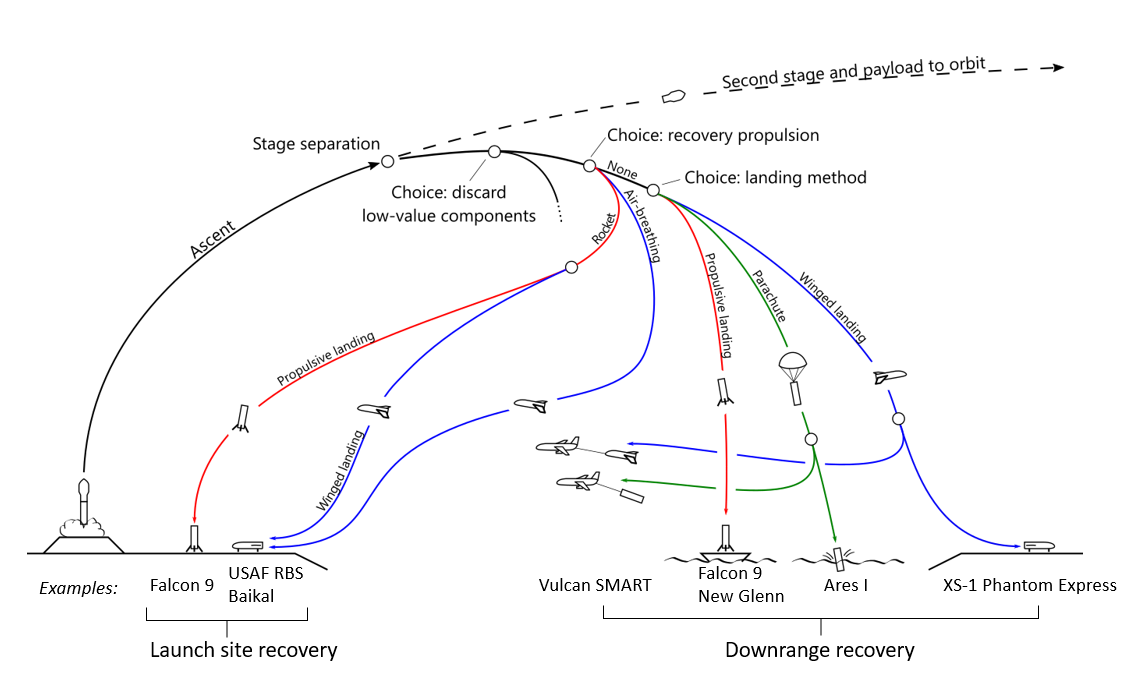
\includegraphics[width=1\textwidth]{figures/recovery_options_annotated}
    \caption{\label{fig:recov_strat_diagram} Many different strategies can be employed to recover and reuse the \nth{1} stage of a launch vehicle.}
\end{figure*}

The following sections will estimate the performance and cost per flight of several of the above reuse strategies.

\section{Performance Model}

Overall payload mass fraction is the key performance metric for launch vehicles. It determines how large a vehicle is needed to launch a given payload. As larger launch vehicles are generally more expensive, higher payload mass fractions are preferable. This section describes a quick method for estimating the payload capacity of 2-stage launch vehicles with reusable first stages, suitable for preliminary concept evaluation.

The payload mass fraction $\pi_*$ is defined as:

\begin{equation}
\pi_* \equiv \frac{m_*}{m_0}
\end{equation}

where $m_*$ is the (maximum) payload mass and $m_0$ is the gross (wet) liftoff mass of the vehicle, including payload, all stages and propellant.

Payload performance depends on the target orbit and on the design of the launch vehicle. The relation between vehicle design, payload capacity, and the $\Delta v$ required to reach the target orbit is expressed by Tsiolkovsky’s rocket equation. The $\Delta v$ capability of a single stage is\footnote{The form of Tsiolkovsky's equation used here is taken from \cite{Wiesel2010}}:

\begin{equation}
\Delta v_i = - I_{sp,i} g_0 \ln \left( \epsilon_i + (1 - \epsilon_i) \pi_i \right)
\end{equation}

where $I_{sp,i}$ is the (altitude-averaged) specific impulse of the $i$-th stage engines, $\epsilon_i$ is the inert mass fraction of the $i$-th stage, and $\pi_i$ is the payload mass fraction of the $i$-th stage. The inert mass fraction is the stage's inert mass divided by its wet mass:

\begin{equation}
\epsilon_i \equiv \frac{m_{inert,i}}{m_i} = \frac{m_{inert,i}}{m_{inert,i} + m_{p,i}}
\end{equation}

The payload mass fraction of a \emph{stage} is:
\begin{equation}
\pi_i \equiv \frac{\sum_{j=i+1}^N (m_j) + m_*}{m_i + \sum_{j=i+1}^N (m_j) + m_*}
\end{equation}

where $\sum_{j=i+1}^N (m_j) + m_*$ is the mass of the upper stages and payload carried by stage $i$.

For a two stage launch vehicle, we introduce an additional parameter, $y$, the stage 1 / stage 2 wet mass ratio:

\begin{equation}
y \equiv \frac{m_2}{m_1}
\end{equation}

For current U.S. 2-stage launch vehicles, values of $y$ are 0.076 to 0.265. Lower values of $y$ result in a higher staging velocity for a given mission and there is a value of $y$ which maximizes $\pi_*$ if the other parameters are fixed.

Then, for two-stage vehicles, Tsiolkovsky’s relation can be written as the following system of equations:

\begin{equation}
\begin{aligned}
% TODO multiline equation align equals signs
\label{eq:dv_2_stage}
\Delta v_* &= \Delta v_1 + \Delta v_2 \\
           &= - I_{sp,1} g_0 \ln \left( \epsilon_1 + (1 - \epsilon_1) \pi_1 \right) \\
             & \quad - I_{sp,2} g_0 \ln \left( \epsilon_2 + (1 - \epsilon_2) \pi_2 \right)
\end{aligned}
\end{equation}

\begin{equation}
\label{eq:ypi}
\pi_2 = (y + 1) - \frac{y}{\pi_1}
\end{equation}

\begin{equation}
\label{eq:pi_prod}
\pi_* = \pi_1 \pi_2
\end{equation}

A given launch vehicle design is represented by the parameters $(I_{sp,1}, I_{sp,2}, \epsilon_1, \epsilon_2, y)$. Given these parameters and a target orbit, we find the payload performance of the launch vehicle by:

\begin{enumerate}
    \item fixing $\Delta v_*$ to the $\Delta v_*$ required to reach the target orbit from the launch site, including losses.
    \item solving (numerically) the system of equations (\ref{eq:dv_2_stage}-\ref{eq:pi_prod}) for $\pi_*$
\end{enumerate}

To validated the model, calculations were run for the Delta IV Medium and Falcon 9 Block 3 (expendable configuration) launch vehicles [Figure \ref{fig:payload_vs_dv}]. The advertised payload mass fractions for LEO and GTO are shown (crosses) for comparison. The model slightly over-predicts $\pi_*$, likely because it neglects the mass of the payload fairing.

\subsection{Technology choice}
Clearly, payload performance depends on inert mass fraction and specific impulse, and would be maximized for $\epsilon \rightarrow 0, \quad I_{sp} \rightarrow \infty$. However, there are technological limits on the achievable values, which depend on a collection of design decisions, i.e. the propellant, engine cycle, tank and structure materials, etc. We refer to this collection of decisions as a "technology choice". The technology choice sets $I_{sp, 1}, I_{sp, 2}$, and sets lowers feasible limits for the inert mass fractions, which we will call $E_1, E_2$. The technology choice also influences the cost model (see next section). We will analyze reuse strategies under two example technology choices:

\begin{itemize}
    \item \ce{H2} / \ce{O2} propellants, staged combustion cycle, aluminum alloy tanks
    \item kerosene / \ce{O2} propellants, gas generator cycle, aluminum alloy tanks
\end{itemize}

These technologies are mature and have had fairly consistent specific impulse and inert mass limits over the past 30 years\footnote{This analysis can easily be extended to new technologies, e.g. \ce{CH4} / \ce{O2} propellants or composite tanks, as the engineering limits on these technologies emerge}. Stages using hydrogen technology have higher $I_{sp}$ but higher feasible inert mass $E$ than those using kerosene. The balance of these effects works out to slightly favor hydrogen in terms of payload performance [Figure \ref{fig:payload_vs_dv}]. Finally, note that the technology choice and reuse strategy are independent - any reuse strategy can conceivably be used with any technology choice.

\begin{figure}[H]
    \centering
    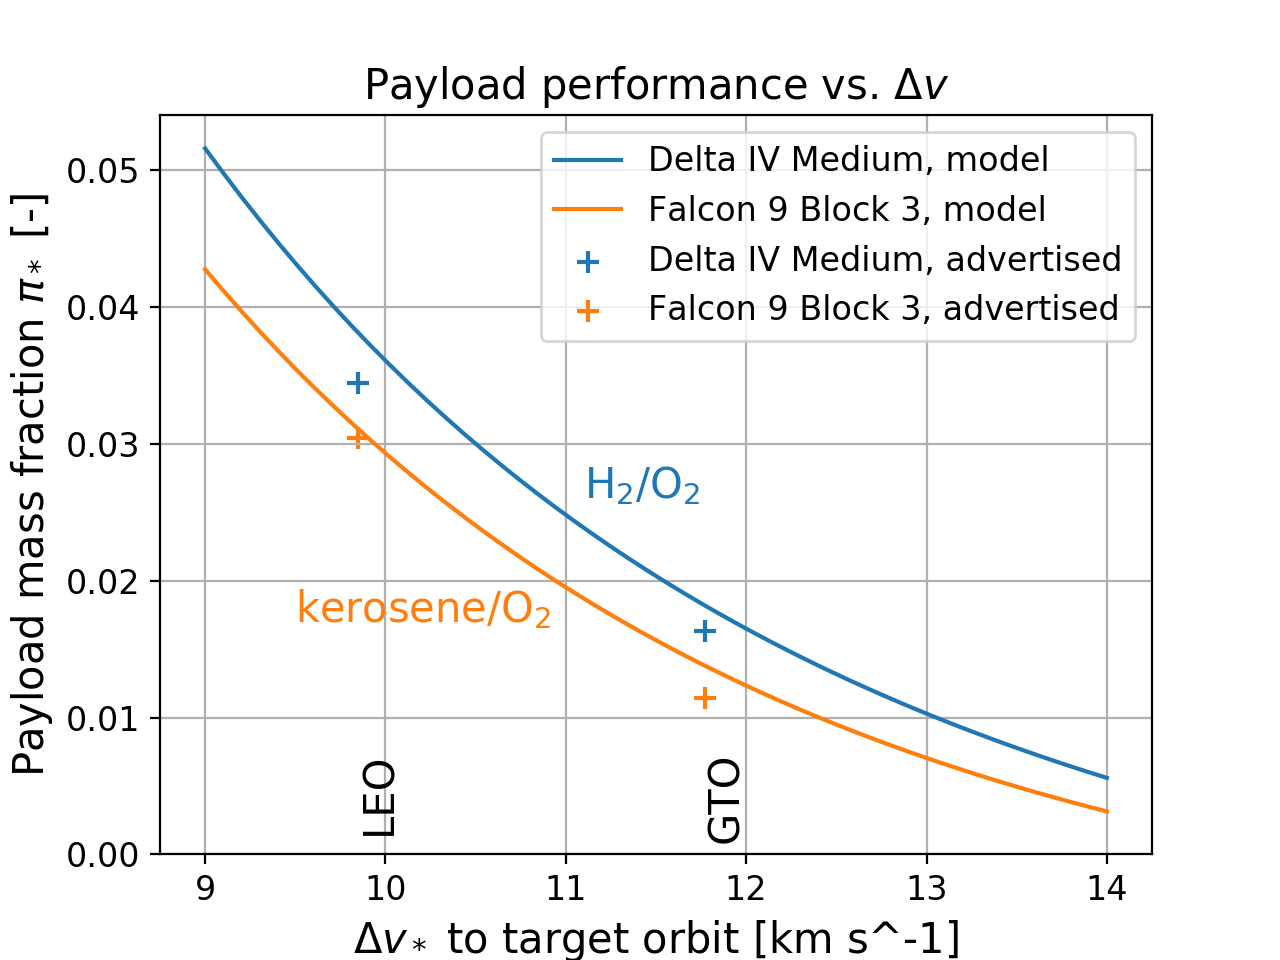
\includegraphics[width=0.5\textwidth]{../../lvreuse/analysis/performance/plots/payload_vs_dv}
    \caption{\label{fig:payload_vs_dv} The quick model makes reasonably accurate predictions of the payload capacity of two expendable launch vehicles. Payload performance declines with increasing $\Delta v_*$, and is slightly higher for \ce{H_2} fueled vehicles than for kerosene vehicles.}
\end{figure}

\subsection{How first stage reuse effects performance}
So far we have reviewed the factors determining launch vehicle performance. Now we ask, how does first stage reuse change these factors? Two mechanisms are possible:

\begin{itemize}
    \item \emph{$\Delta v$ losses} - Some reuse strategies require modifying the outer mold line of the stage or altering the ascent trajectory. This changes the drag, gravity and steering losses during ascent, and could cause the $\Delta v_*$ to a target orbit to be different for reusable and expendable strategies.
    \item \emph{Extra mass on the first stage} - All reuse strategies require the first stage to carry some extra mass during ascent, as extra hardware (landing gear, wings, etc.) and/or as propellant reserved for recovery.
\end{itemize}

The first can be ignored, as the variation of losses for different recovery strategies is minor and comparable to the variation in losses for fully expendable vehicles \cite{Stappert2017}. Thus, the main effect of first stage reuse on performance is that extra mass must be carried during ascent.

\begin{figure*}
    \centering
    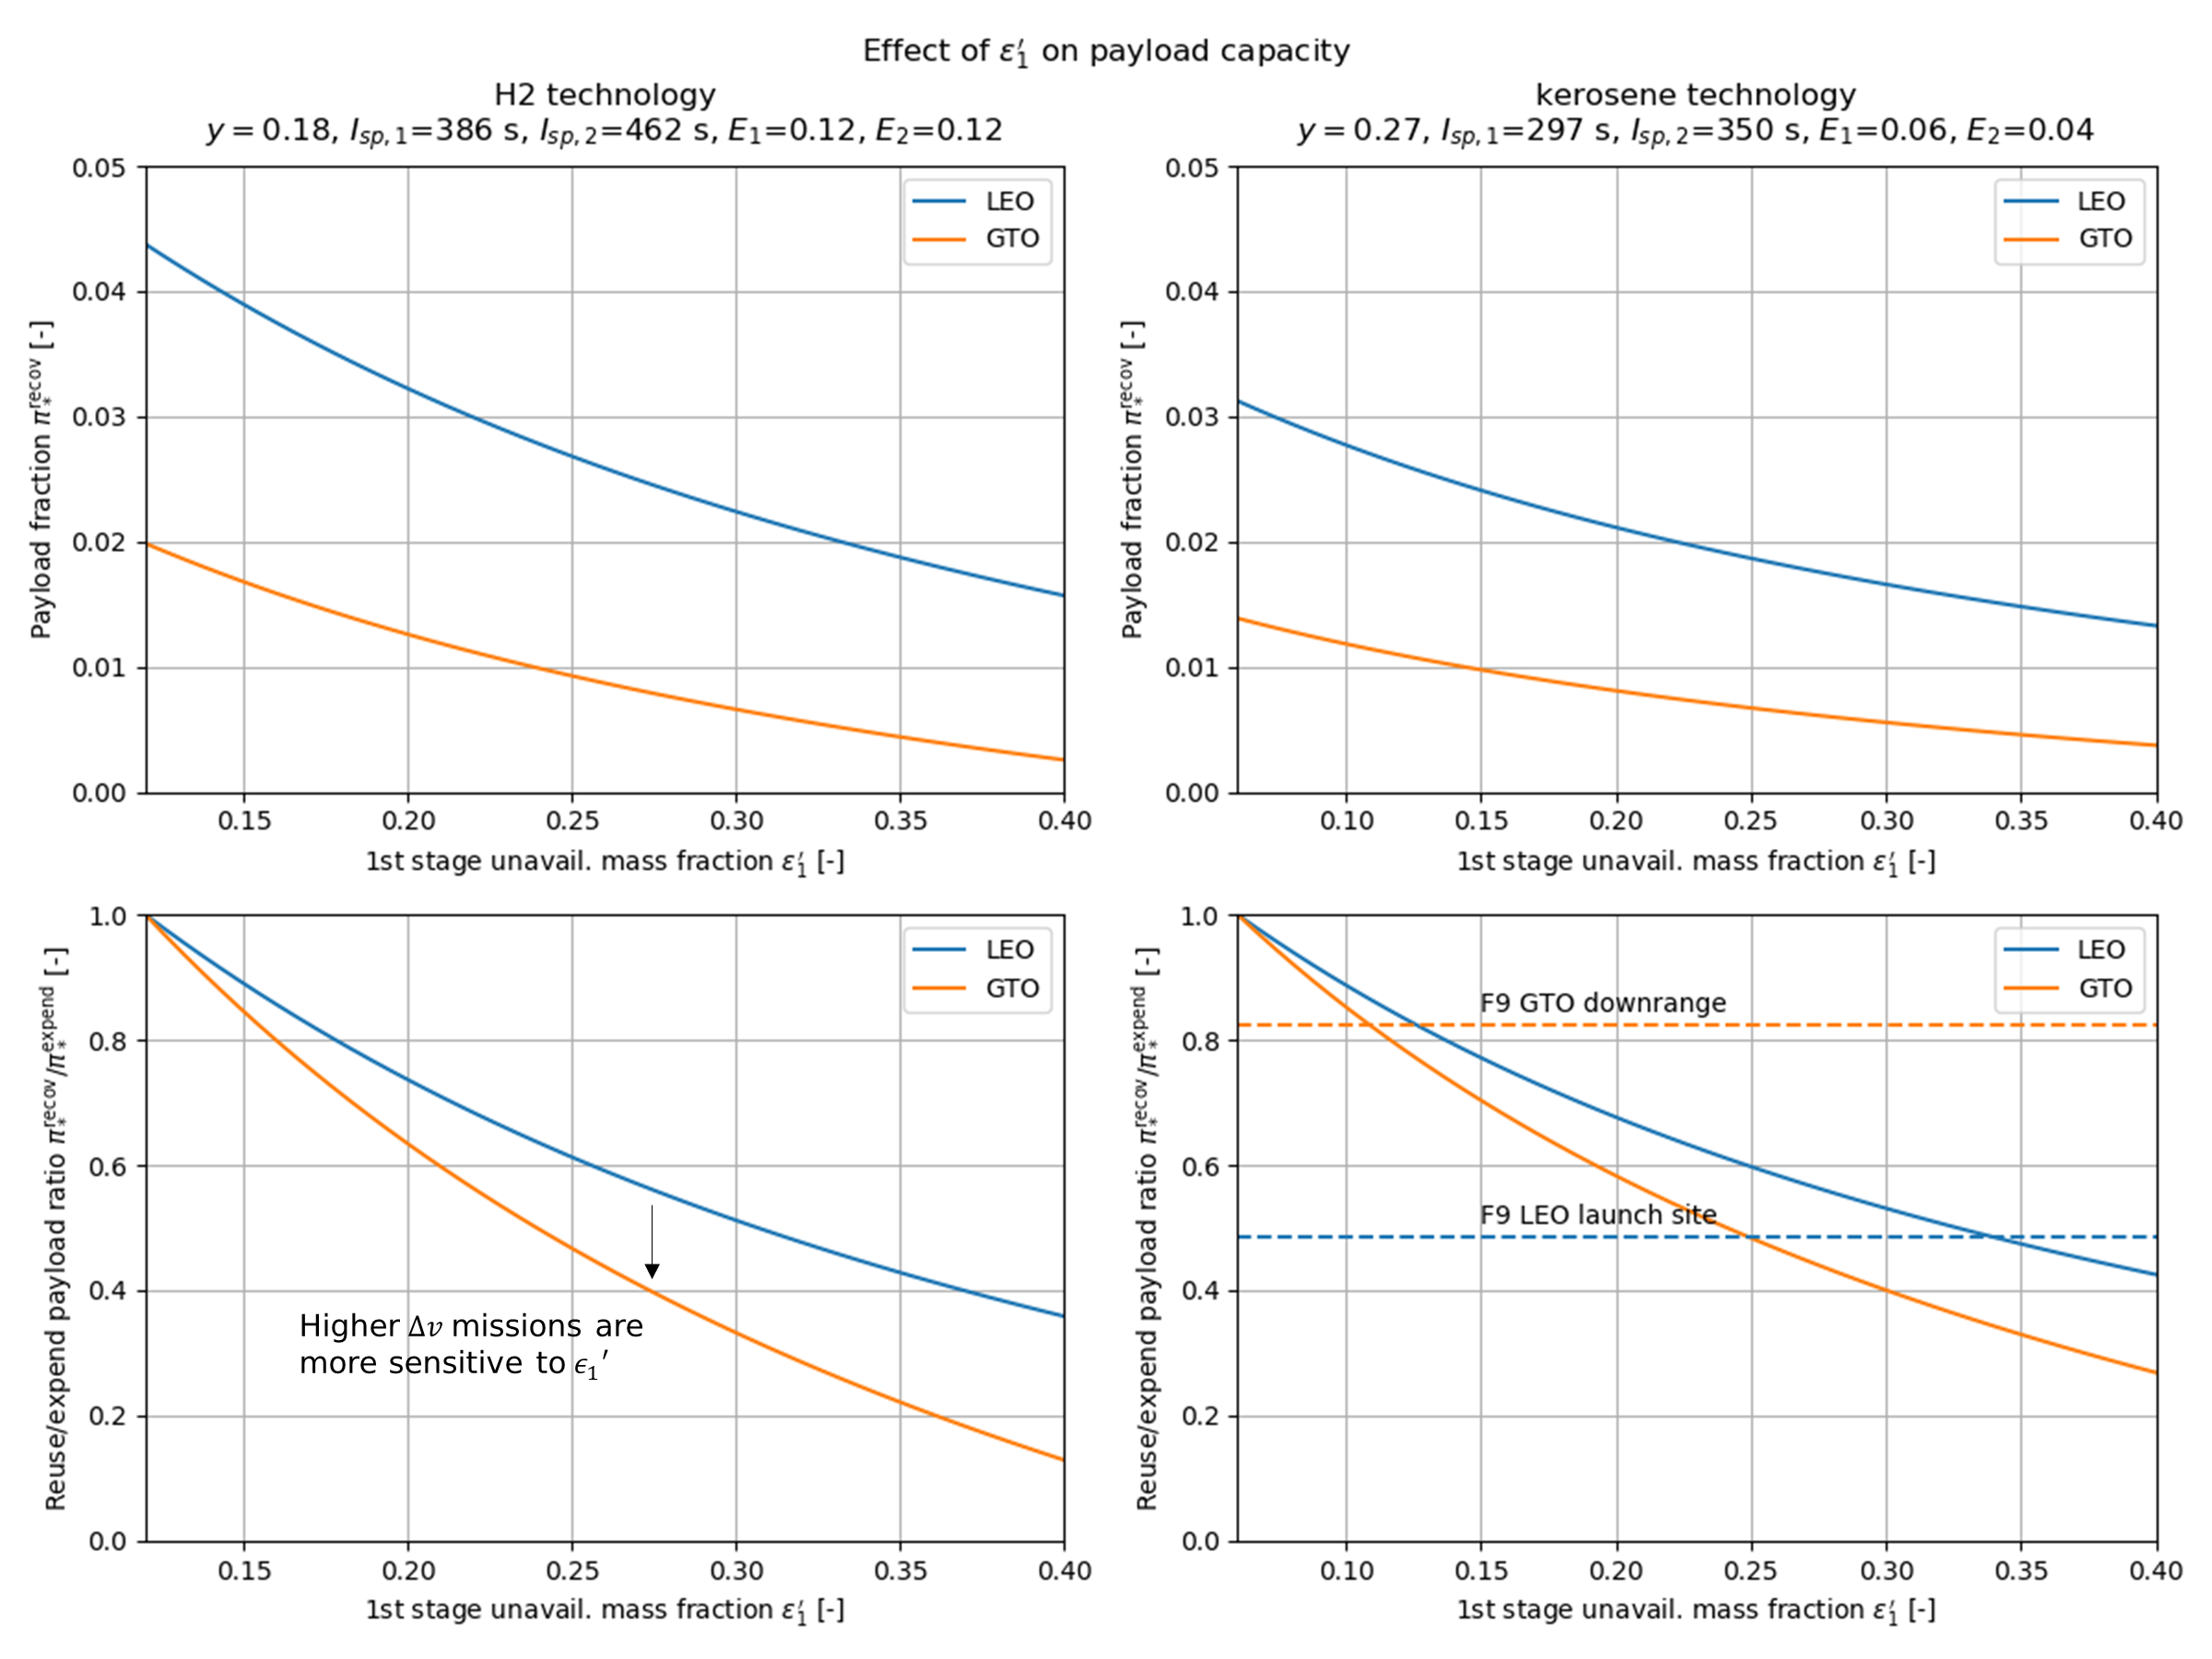
\includegraphics[width=\textwidth]{payload_vs_unavail_mass_annotated}
    \caption{\label{fig:payload_vs_unavail_mass} Payload performance declines as first stage unavailable mass increases.}
\end{figure*}

\subsection{First stage unavailable mass}
We define the "first stage unavailable mass fraction", $\epsilon_1'$, to be the fraction of first stage gross mass that is unavailable to be expelled during ascent, i.e.:

\begin{equation}
\label{eq:epsilon_1_prime}
\epsilon_1' = \frac{m_{inert,1} + m_{pr,1}}{m_{inert,1} + m_{p,1}} = \frac{m_{inert,1} + m_{pr,1}}{m_1}
\end{equation}

where $m_{pr,1}$ is the mass of propellant reserved for recovery maneuvers, and $m_{p,1}$ is the total stage 1 propellant mass.
The payload performance of a vehicle with first stage reuse can be found by substituting $\epsilon_1'$ for $\epsilon_1$ in Equation \ref{eq:dv_2_stage}, and solving Equations \ref{eq:dv_2_stage}-\ref{eq:pi_prod}.

Note that all reuse strategies add unavailable mass to the first stage, so we will always have $\epsilon_1' > E_1$.

The effect of first stage unavailable mass on payload performance is shown in Figure \ref{fig:payload_vs_unavail_mass}. The top plots show the overall payload mass fraction as a function of $\epsilon_1'$. The bottom plots show the payload capacity of a vehicle with first stage reuse as a fraction of the payload capacity of an "equivalent" expendable vehicle with the minimum feasible first stage inert mass fraction $E_1$. Note that the same $\epsilon_1'$ causes a larger fractional reduction of payload capacity on higher $\Delta v$ missions.

\subsection{Relating unavailable mass to recovery hardware and propulsion}
Next, we relate $\epsilon_1'$ to the feasible limit on inert mass ($E_1$) and the extra hardware and propellant needed for recovery.
It will be helpful to compare the inert mass of the first stage to a "baseline" hardware mass:

\begin{equation}
m_{hb,1} \equiv \frac{E_1}{1 - E_1} m_{p,1}
\end{equation}

i.e. the mass that the first stage would have if it were build to lightest limit feasible for an expendable vehicle. We can think of this as the mass of the baseline hardware that would be present on an expendable first stage, i.e. tanks, rocket engines and thrust structure. In addition to the baseline mass, a reusable stage will have some additional recovery hardware (e.g. wings, landing gear, parachutes) with mass $m_{hr,1}$. Thus, for a reusable stage $m_{inert,1} = m_{hb,1} + m_{hr,1}$.

Then, we define three new dimensionless variables:
\begin{itemize}
    \item $z_m \in (0, 1]$ is the fraction of the first stage baseline mass which is recovered, i.e.
    \begin{equation}
    z_m \equiv \frac{m_{hv,1}}{m_{hb,1}}
    \end{equation}
    where $m_{hv,1}$ is the mass of the valuable hardware to be recovered. For full reuse of the first stage $z_m = 1$. If only an engine pod is recovered, $z_m \approx 0.3$.

    \item $H \in (0, 1)$ is the recovery hardware factor; the mass of the recovery hardware divided by the dry mass of the recovered stage or pod:
    \begin{equation}
    H \equiv \frac{m_{hr,1}}{m_{hr,1} + m_{hv,1}}
    \end{equation}
    The extreme $H=0$ represents the (rather miraculous) situation in which we could recover the valuable hardware without any additional recovery equipment. The extreme $H \rightarrow 1$ represents the situation in which the recovery construction is very poor, and many tons of wings, parachutes, etc. are needed to recover a few kilograms of high-value hardware.

    \item $P \in (0, \infty)$  is the recovery propellant factor. The propellant mass needed for recovery is
    \begin{equation}
    m_{pr,1} = (m_{hr,1} + m_{hv,1}) \left( e^P - 1 \right)
    \end{equation}
    If the recovery maneuvers use rocket propulsion, then $P$ is found from the Tsiolkovsky equation:
    \begin{equation}
    \label{eq:rocket_p}
    P = \frac{\Delta v_r}{g_0 I_{sp,1}}
    \end{equation}
    where $\Delta v_r$ is the $\Delta v$ of the recovery maneuvers. If instead the stage flies back and uses air-breathing propulsion to maintain steady level flight, then $P$ is found from the Berguet range equation:
    \begin{equation}
    \label{eq:berguet_p}
    P =  \frac{R_{\mathrm{cruise}}}{v_{\mathrm{cruise}} (L/D) I_{sp}^{ab}}
    \end{equation}
    where $R_{\mathrm{cruise}}$ is the cruise range, $v_{\mathrm{cruise}}$ is the cruise speed, $(L/D)$ is the cruise lift to drag ratio and $I_{sp}^{ab}$ is the specific impulse of the air breathing engine. If no (mass-expelling) propulsion is used during recovery, $P = 0$ and $m_{pr,1} = 0$.
\end{itemize}

It can be shown that (see appendix TODO):

\begin{equation}
\label{eq:eps_h_p_z}
\epsilon_1' = \frac{1 + \frac{H z_m}{1 - H} +  \frac{z_m}{1 - H} (e^P - 1) }{1 + \frac{H z_m}{1 - H} + \frac{1 - E_1}{E_1} }
\end{equation}

For full recovery ($z_m = 1$) this simplifies to:
\begin{equation}
\epsilon_1' = \frac{e^P}{1 + (1 - H) \left( \frac{1 - E_1}{E_1} \right)}
\end{equation}

Note that $\epsilon_1'$ increases monotonically with $z_m, H$ and $P$; i.e. recovering more of the stage, using more recovery hardware or using more recovery propellant all increase the unavailable mass.

Now, we can estimate the unavailable mass of the first stage (and therefore the launch vehicle payload performance) from the portion of the stage recovered ($z_m$) and estimates of the hardware ($H$) and propulsion ($P$) required by the selected recovery strategy. 

\subsection{Estimating hardware and propulsion for recovery strategies}
In this subsection, we establish estimates of the recovery hardware factor $H$ and propellant factor $P$ for various recovery strategies.

We account for uncertainty in our model using Monte Carlo techniques. In a preliminary design we do not know enough details to make point estimates of $H$, $P$ and the other model input parameters. Instead, we estimate the credible range that each the model input parameter could lie in, and fit probability distributions to these estimates. We then draw many random samples from the input distribution and evaluate our model on each sample to generate a population of model outputs. This population then represents the range of values that the model output can be expected to take on.

A brief summary of the input parameter distributions is given below; more detail is given in appendix TODO.

We estimate $H$ by examining the mass breakdowns of detailed design studies for some types of reusable boosters \cite{Healy1998, Isakowitz2004, Sippel2003, Hellman2005}, and by analogy to the mass breakdowns of other aerospace vehicles. The resulting estimates are summarized in Table \ref{tab:hardware_factor_distributions}.

% TODO fix table

\begin{table}[H]
    \centering
    \caption{\label{tab:hardware_factor_distributions} Uncertainty distribution parameters of the recovery hardware factor $H$. $H$ can run from 0 to 1, higher values of $H$ indicate that more recovery hardware is needed.}
    \begin{tabular}{l l c c c}
    \hline
     & \multicolumn{3}{c}{Triangular dist. params.} \\
     & Min & Mode & Max \\
    \hline
    \hline
    Winged, Glider  & 0.380 & 0.426 & 0.540 \\
    Winged, Air-breathing & 0.490 & 0.574 & 0.650 \\
    \hline
    Propulsive landing  & 0.09 & 0.14 & 0.19 \\
    \hline
    Parachutes & 0.050 & 0.065 & 0.080 \\
    Parachutes and & 0.150 & 0.170 & 0.190 \\
    inflatable heat shield & & & \\
    \hline
    \end{tabular}
\end{table}

We do not estimate $P$ directly; rather we assume distributions on the factors determining $P$. For propulsive landing, these are the $\Delta v$ of the entry burn (which could be \SIrange{0}{1000}{\meter\per\second}), and the $\Delta v$ of the landing burn (which depends on the stage's ballistic coefficient and the landing burn acceleration) [Figure \ref{fig:propulsive_landing}]. For winged stages with air-breathing propulsion, these factors are the lift/drag ratio (4 to 8), air breathing engine specific impulse (\SIrange{3200}{4000}{\second}), and cruise speed (\SIrange{100}{300}{\meter\per\second}) during the powered cruise portion of the return trajectory [Figure \ref{fig:flyback_trajectory}].

% TODO do we really need these figures here?
\begin{figure}[H]
    \centering
    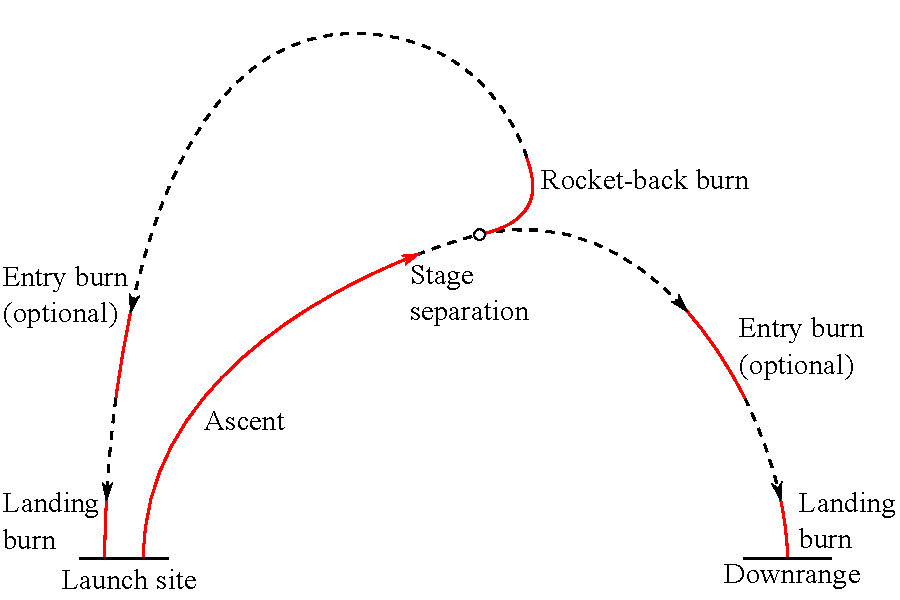
\includegraphics[width=0.5\textwidth]{propulsive_landing}
    \caption{\label{fig:propulsive_landing} Propulsive landing: trajectory options for launch site and downrange recovery. Propulsive portions of the trajectory are shown as red solid lines.}
\end{figure}

\begin{figure}[H]
    \centering
    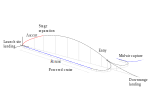
\includegraphics[width=0.5\textwidth]{flyback_trajectory}
    \caption{\label{fig:flyback_trajectory} Winged landing: trajectory options for launch site and downrange recovery. Portions of the trajectory flown under rocket propulsion are shown as red solid lines; air-breathing propulsion is indicated with blue.}
\end{figure}

For launch site recovery there is a further wrinkle - the stage separation velocity $v_{ss}$ depends on the unavailable mass ($v_ss$ decreases as $\epsilon_1'$ increases). But for return-to-launch-site strategies, the recovery propellant factor $P$ (and therefore $\epsilon_1'$) depends on $v_{ss}$. Thus, for return-to-launch-site strategies, we solve simultaneously for $\pi_*, \epsilon_1'$ and $P$. For rocket propelled return, we compute the impulsive $\Delta v$ needed to place the stage on a ballistic trajectory to the launch site, plus gravity losses. For air-breathing return, we use the Berguet range equation \footnote{In both cases, we model the downrange distance at stage separation as $R = f_{ss} v_{ss}^2$, where $f_{ss}$ is an uncertain coefficient, whose dispersion is calibrated to data from actual launches and detailed trajectory simulations}.

The specific impulses and minimum feasible inert mass fractions are also dispersed. Their distributions are based on data from previous launch vehicles and engines \cite{Isakowitz2004, hist_lpre}. 

These estimates are summarized in Figure \ref{fig:unavail_mass_contours}, which shows contours of $\epsilon_1'$ on $P$ vs. $H$ axes. The likely ranges of $P$ and $H$ for some recovery strategies are shown as blue ellipses. This figure assumes kerosene technology and full recovery of the first stage. Note that the (launch site, rocket-propelled, propulsive landing) strategy incurs the highest unavailable mass because of the large amount of propellant required to return the stage to the launch site. The (downrange, no propulsion, parachute landing) strategy has the lowest unavailable mass. 

\begin{figure}[H]
    \centering
    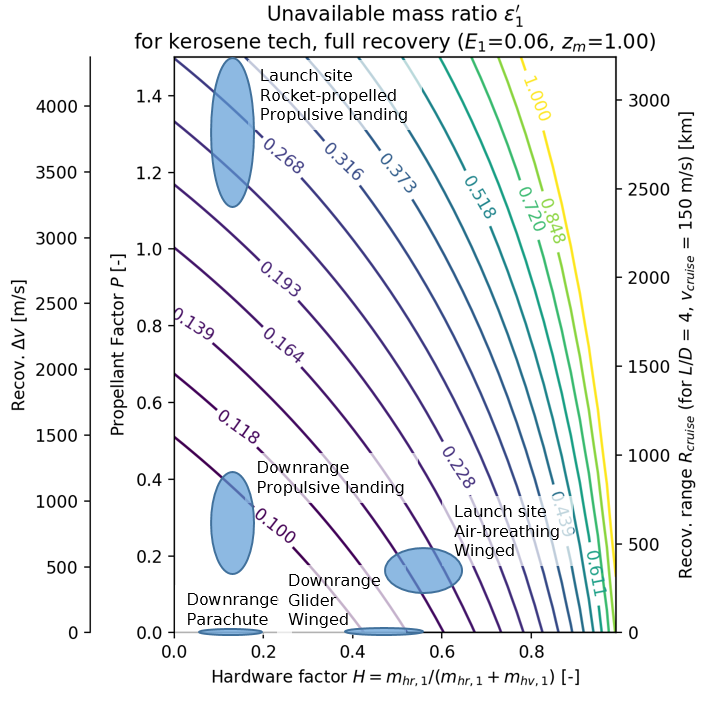
\includegraphics[width=0.5\textwidth]{unavail_mass_contours_annotated}
    \caption{\label{fig:unavail_mass_contours} Contours of unavailable mass versus the recovery propellant and hardware factors. Credible ranges for some recovery strategies are shown.}
\end{figure}


\subsection{Payload fraction estimates for recovery strategies}
The distributions of payload performance resulting from this model are shown as violin plots in Figures \ref{fig:strategy_perf_kerosene} and \ref{fig:strategy_perf_H2}. A different plot is provided for each combination of technology choice (kerosene, \ce{H2}) and mission (LEO, GTO). First, note the spread of the distribution for a fully expendable vehicle - this indicates the uncertainty due to technology factors ($I_{sp}$ and $E$). We should only consider a reuse strategy to have a meaningful impact on payload performance if most of its $\pi_*$ distribution does not overlap the range of $\pi_*$ that can be expected from an expendable vehicle.

Across all technology choices and missions, the parachute landing strategies have little impact on payload performance, and their difference from the expendable performance is small compared to the range of uncertainty. The (launch site, air-breathing, winged, partial recovery), (downrange, propulsive landing, full recovery), and (downrange, no propulsion, winged, full recovery)  strategies have slightly lower payload performance than expendable, and are almost indistinguishable from each other.  Propulsive landing at the launch site has the worst payload performance; with kerosene on a GTO mission its payload mass fraction is unacceptably low. Across all strategies, reuse causes a larger fractional decrease in $\pi_*$ on the higher-$\Delta v$ mission (GTO).

These payload mass fraction estimates allow us to predict the mass of the launch vehicle required to lift a payload into a target orbit. In the next section, we develop a model that uses the launch vehicle masses, along with other factors, to estimate system cost.

\begin{figure*}
    \centering
    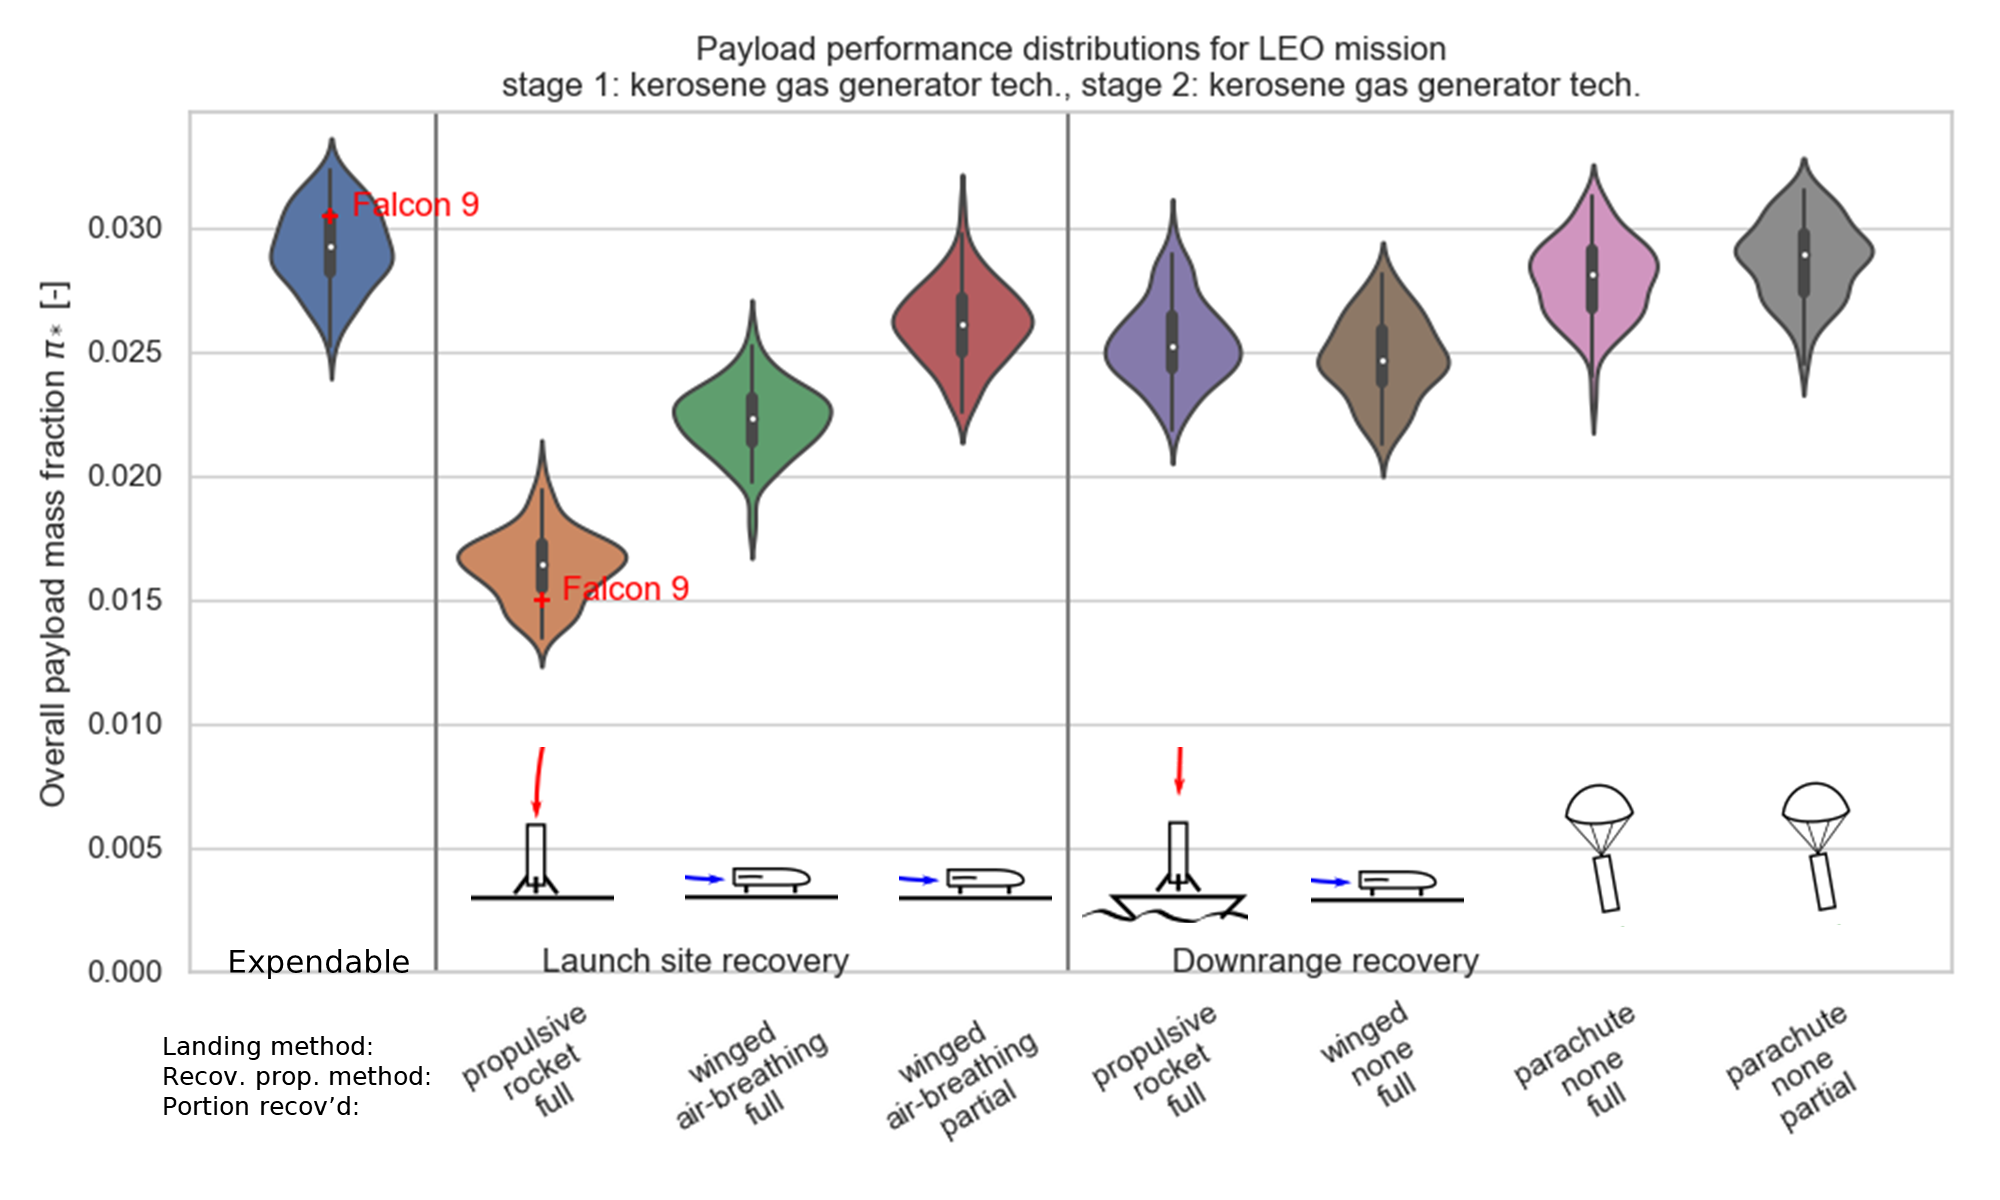
\includegraphics[width=\textwidth]{strategy_perf_annotated/LEO_kero}
    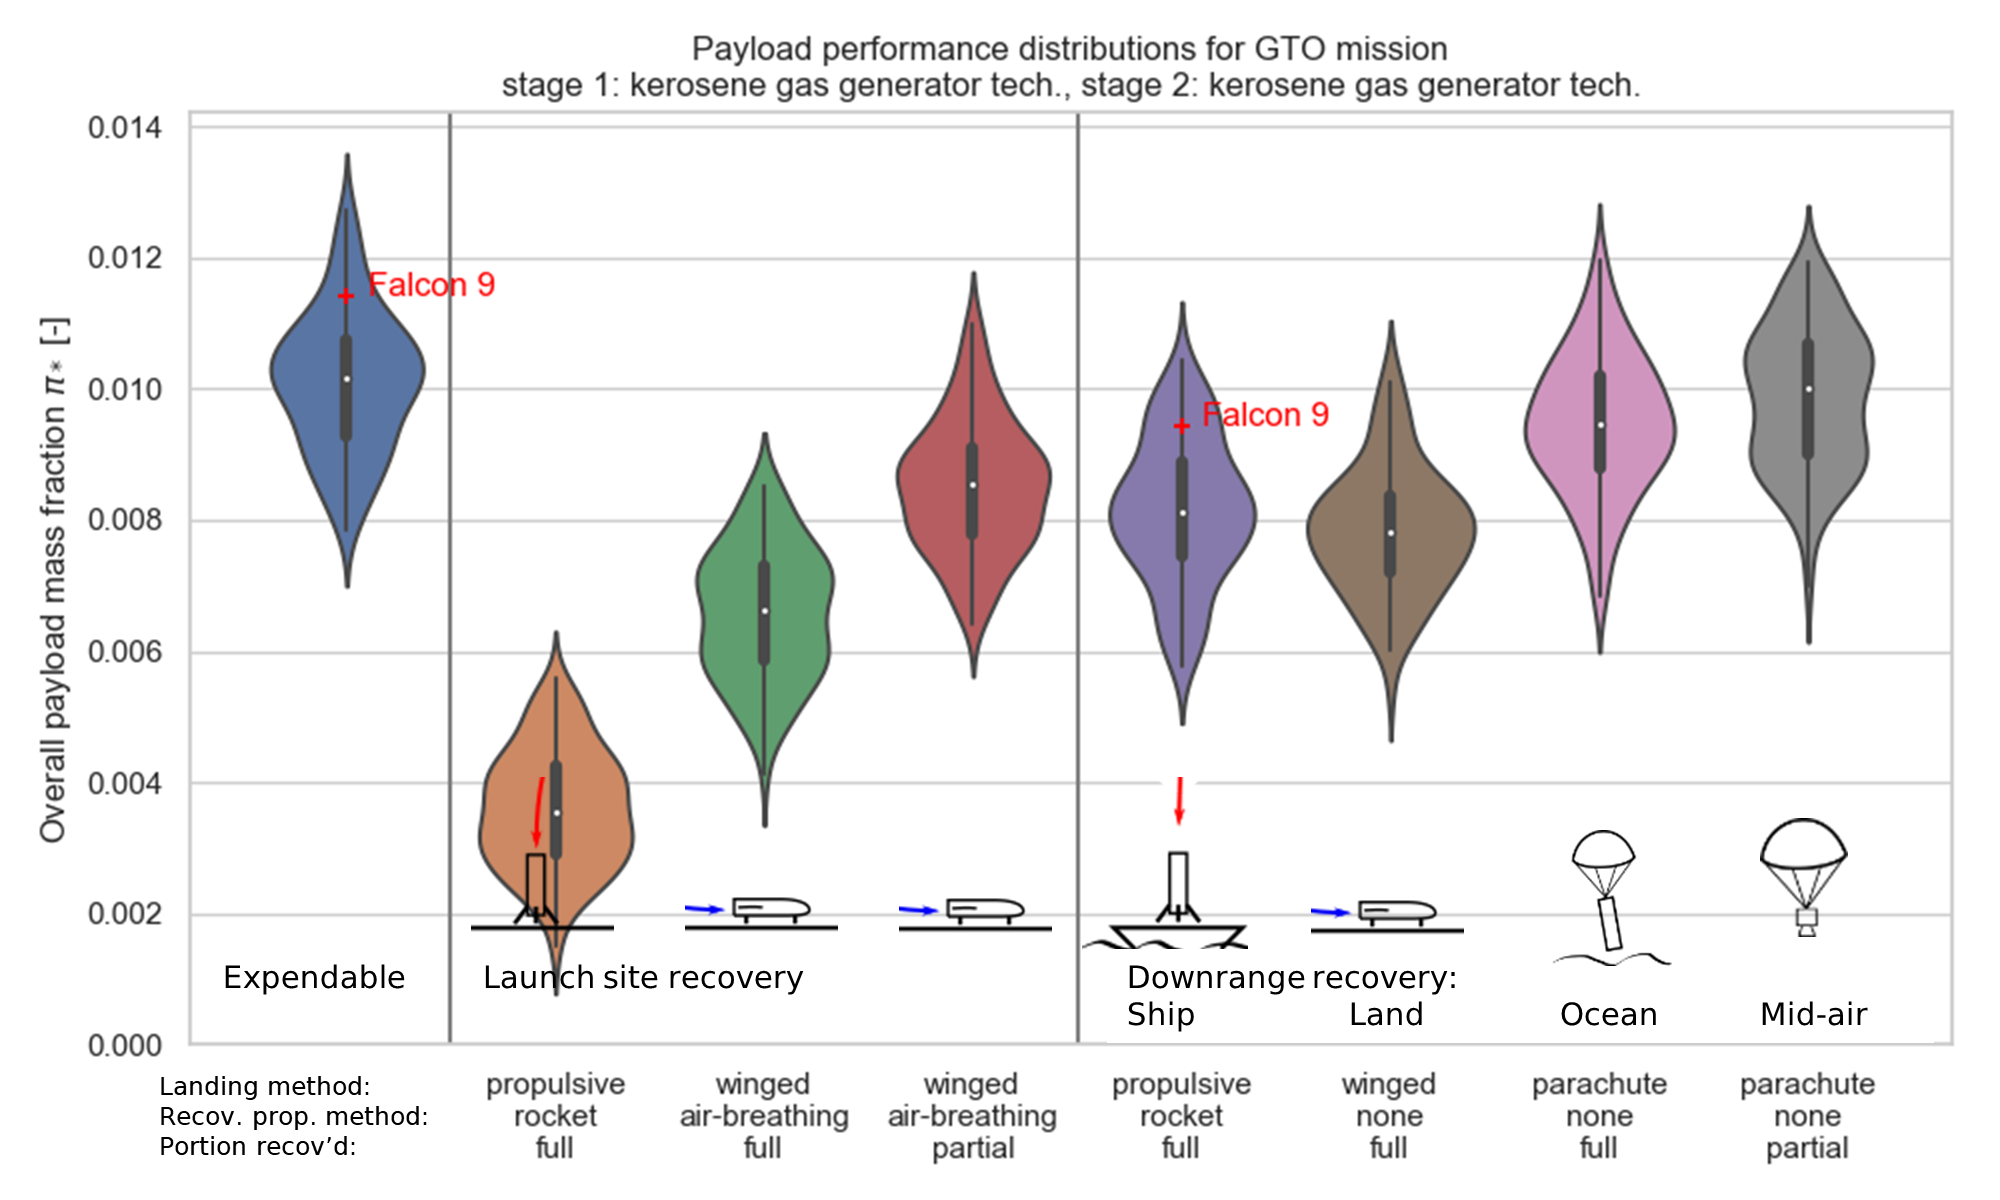
\includegraphics[width=\textwidth]{strategy_perf_annotated/GTO_kero}
    \caption{\label{fig:strategy_perf_kerosene} Distributions of payload performance for various first stage recovery strategies with kerosene technology. Reported payload performance for Falcon 9 block 3 is shown for comparison.}
\end{figure*}

\begin{figure*}
    \centering
    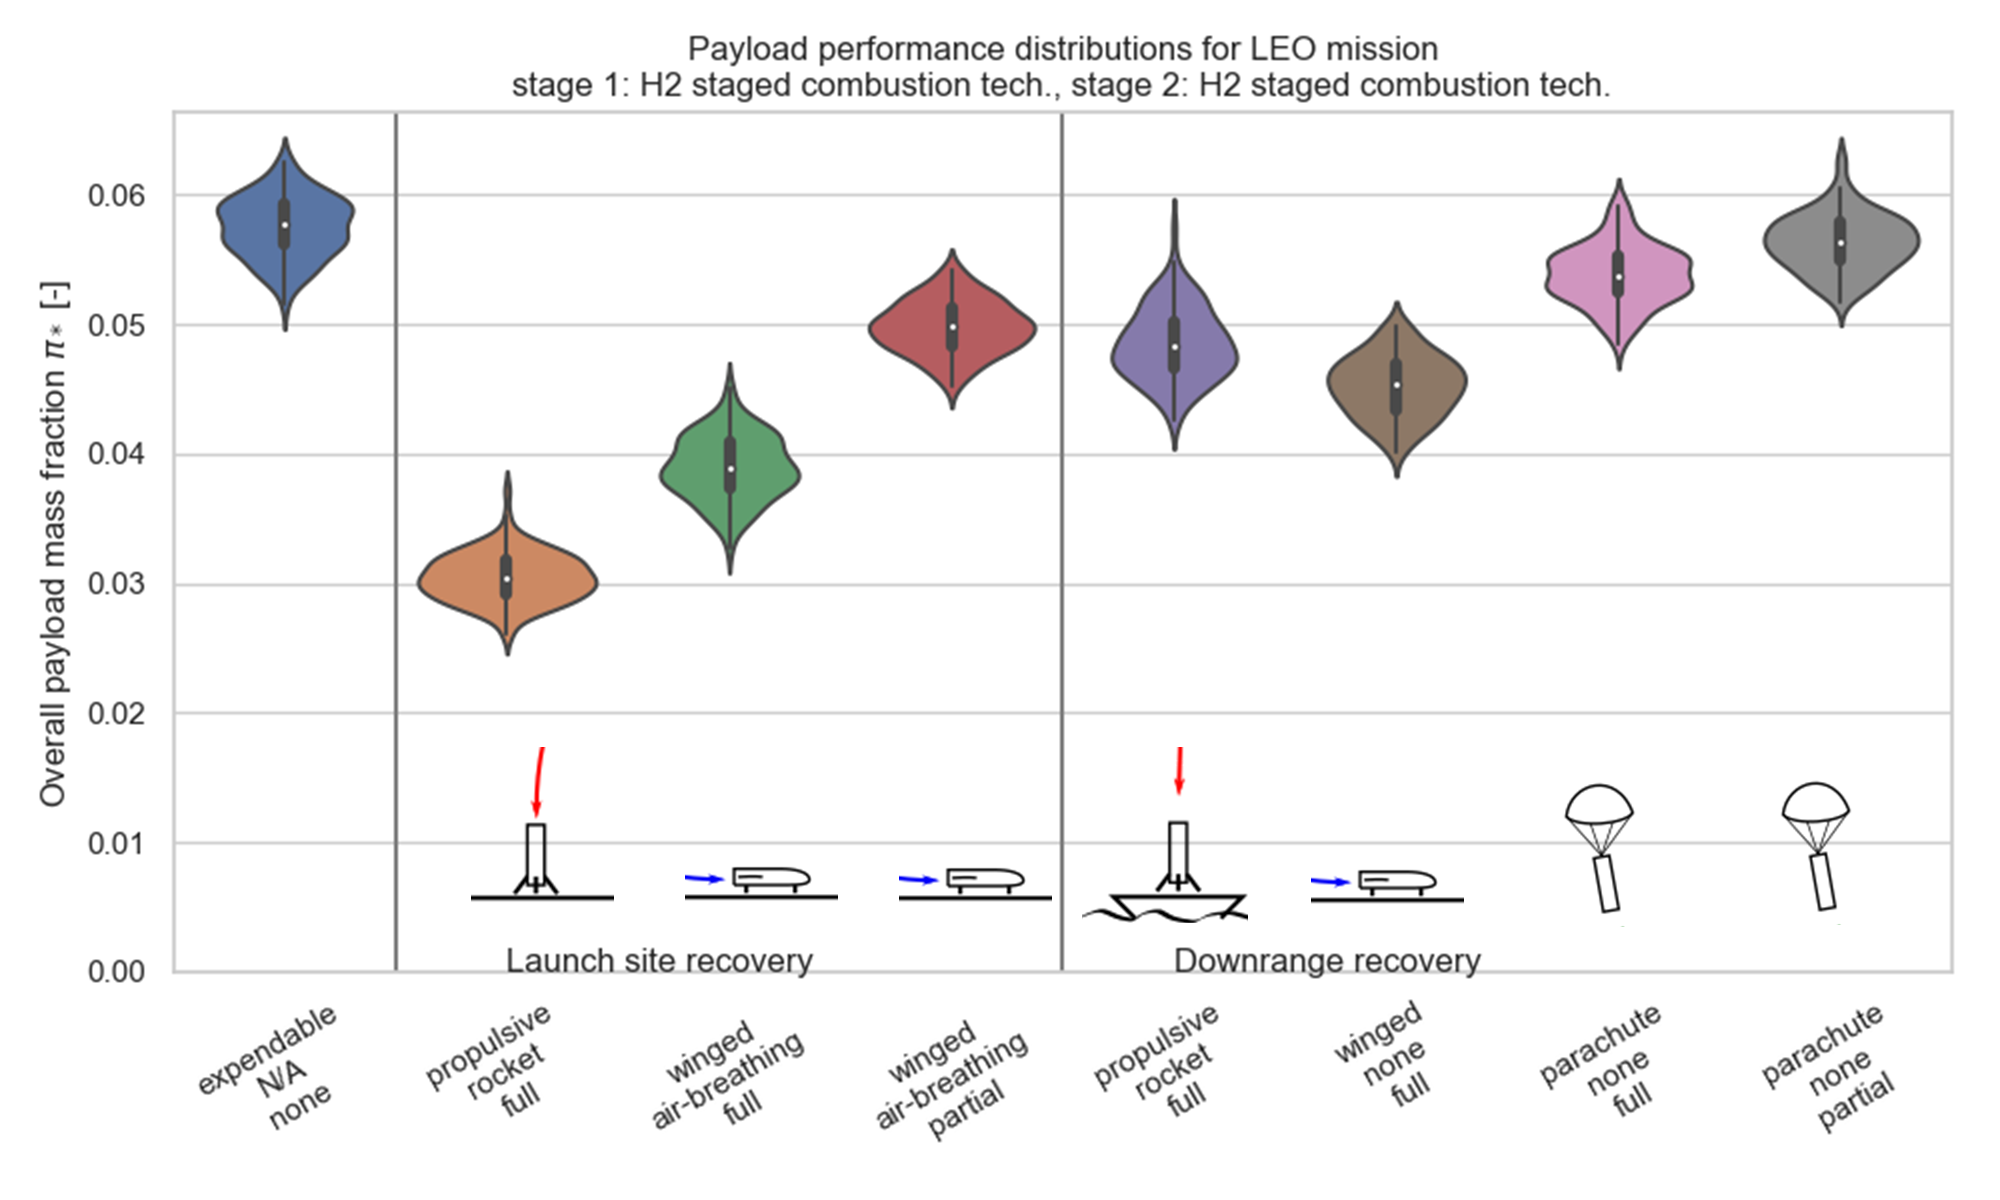
\includegraphics[width=\textwidth]{strategy_perf_annotated/LEO_H2}
    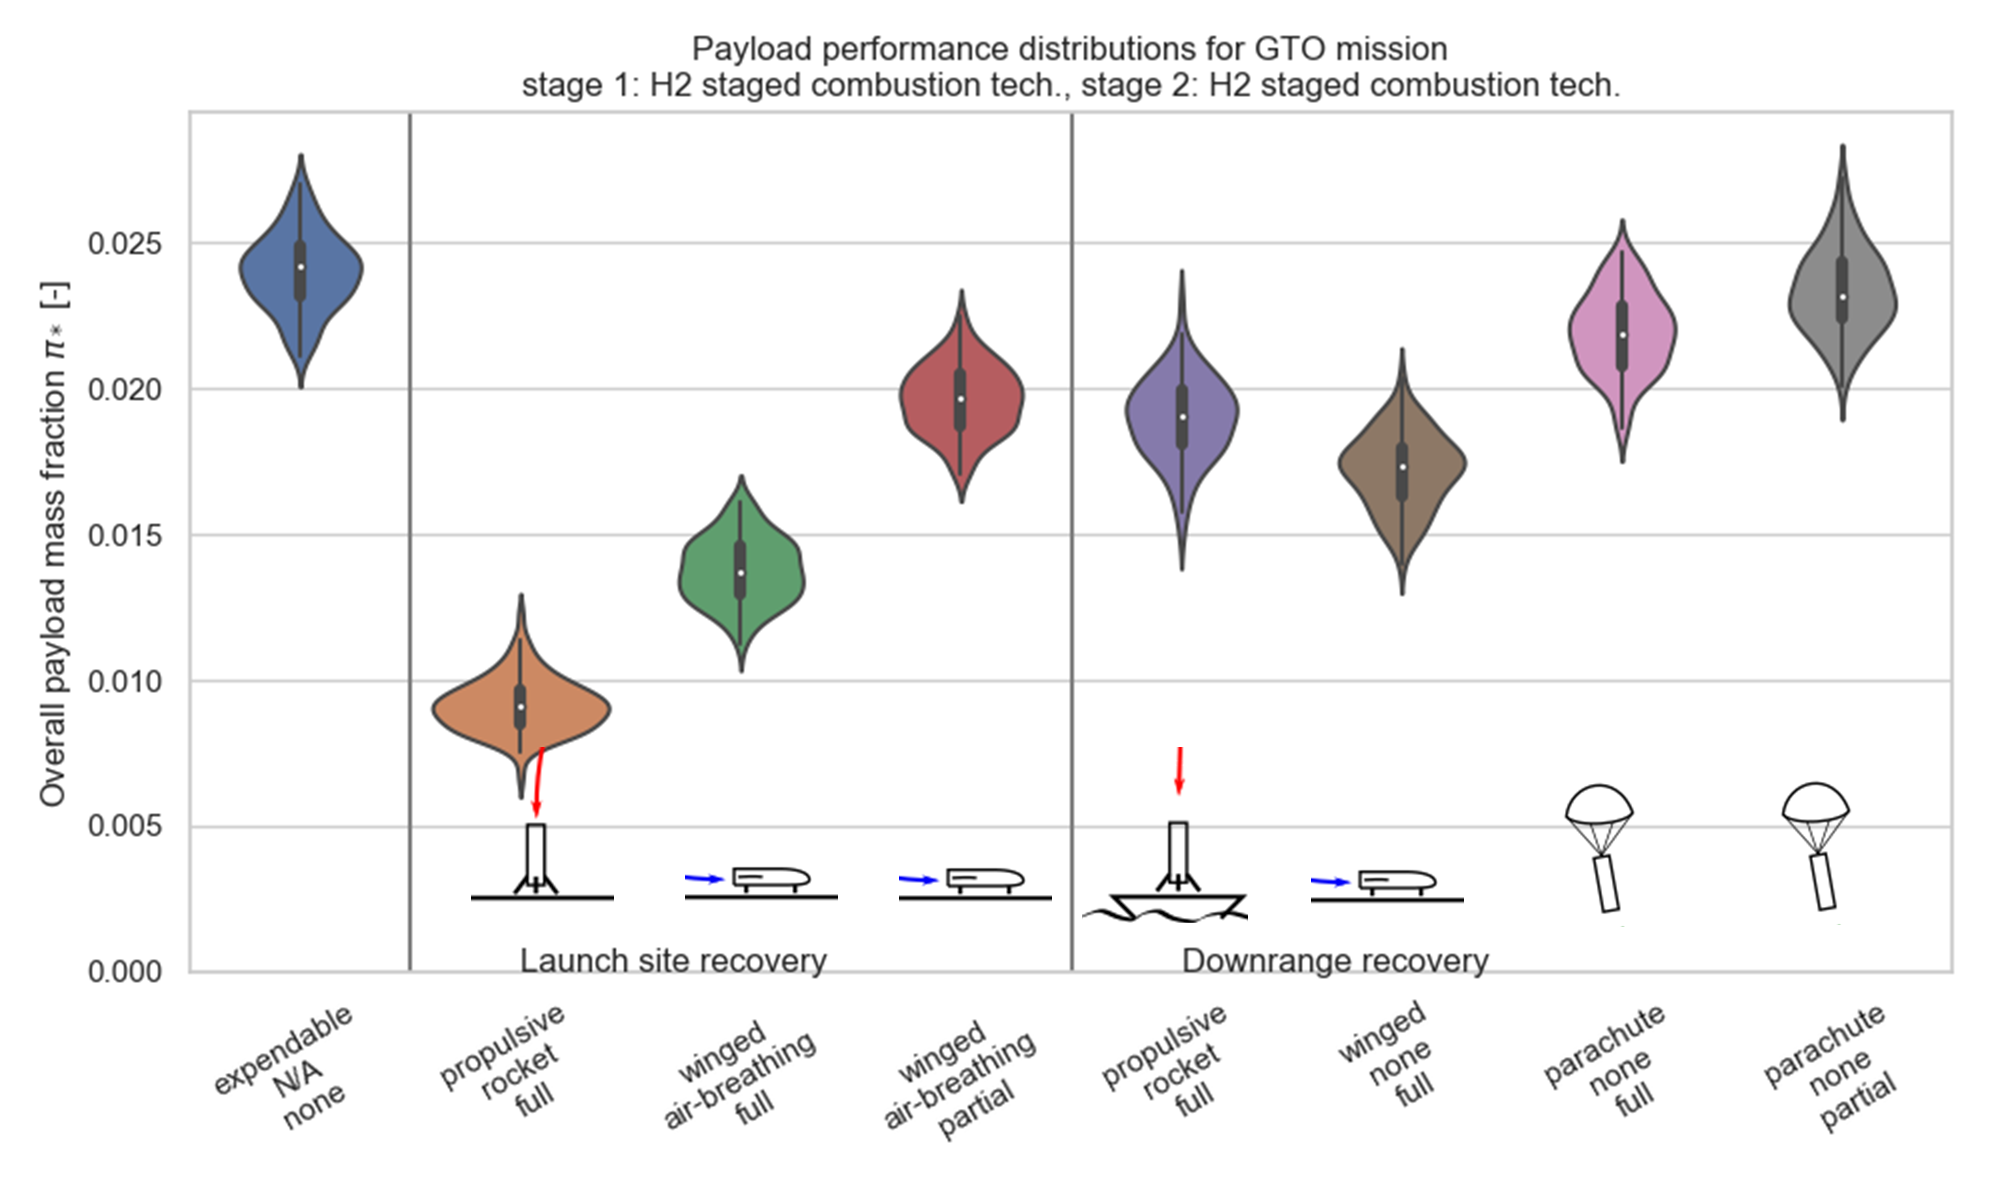
\includegraphics[width=\textwidth]{strategy_perf_annotated/GTO_H2}
    \caption{\label{fig:strategy_perf_H2} Distributions of payload performance for various first stage recovery strategies with \ce{H2} technology.}
\end{figure*}

\section{Cost Model}

The TRANSCOST 8.2 model was implemented to evaluate the costs of different first stage reuse strategies \cite{transcost}. TRANSCOST is a top-down cost estimating model that utilizes historical data for similar projects to estimate the cost of launch vehicle elements. A series of cost estimation relationships (CERs) of the form $C = a M^x$ relate the mass $M$ of launch vehicle elements to their production costs using the empirically fitted parameters $a$ and $x$. Costs of all launch vehicle elements are then summed to determine the total launch vehicle production cost. 

The cost and performance models are linked through the launch vehicle element masses. For a given payload mass, the performance model can estimate the mass of launch vehicle elements for various first stage reuse strategies. These masses are then used with the cost model to estimate the production cost and cost per flight of those strategies. 

\subsection{Cost Model Description}

The TRANSCOST model considers three separate cost areas for launch vehicles: development, production, and operations costs \cite{transcost}. The cost per flight of a launch vehicle is the cost paid by the launch service provider for each flight, which includes production and operations costs only. The price per flight is the price paid by a customer to the launch service provider. This includes production and operations costs, as well as profit for the launch service provider and a potential development amortization charge. It should be noted, however, that typically a large part of development costs are funded by government contracts, such as for the Falcon 9 and Ariane 5 launch vehicles \cite{NASAspaceX, ESAAriane5}. In these cases, a development amortization charge is substantially reduced or not included as part of the price per flight.

It is interesting to look at the breakdown of costs in the cost per flight of a launch vehicle. Consider a two stage fully expendable launch vehicle utilizing kerosene and liquid oxygen propellants to carry a 10,000 kg payload to LEO. The cost per flight breakdown for such a launch vehicle can be seen in Figure \ref{fig:expendable_cost_breakdown}. 

\begin{figure}[H]
    \centering
    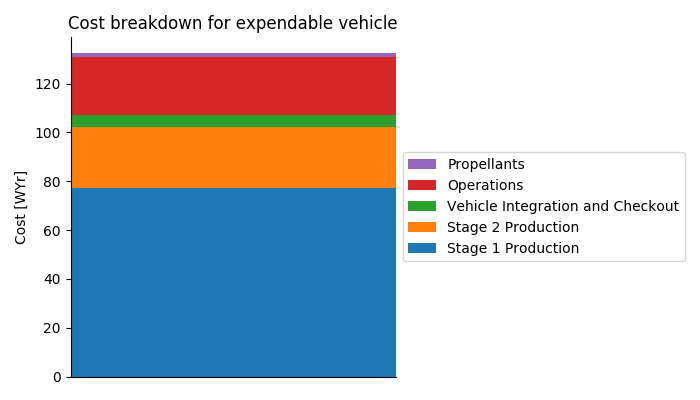
\includegraphics[width=0.5\textwidth]{../../lvreuse/analysis/combined/plots/expendable_cost_breakdown}
    \caption{\label{fig:expendable_cost_breakdown} Cost per flight breakdown for two stage fully expendable vehicle.}
\end{figure}

For this launch strategy -- and similarly for most fully expendable launch vehicle strategies -- the cost per flight is dominated by the first stage production costs. These large first stage production costs motivate strategies for first stage reusability, which would allow the first stage production cost to be amortized over a number of flights, therefore potentially reducing the total cost per flight. 

\subsection{Validation of Cost Model}

In order to validate the TRANSCOST model, the prices per flight for several current launch vehicles were evaluated with the model and compared to their actual advertised launch prices. As with the performance model, uncertainty in the cost model is accounted for using Monte Carlo methods. Credible range estimates for various cost parameters are used to establish parameter distributions. These distributions are then sampled to evaluate the cost model, generating a collection of cost model outputs that represent a range of credible cost estimates.

It should be noted that the TRANSCOST model as published only gives point estimates of launch vehicle costs, and provides no quantification for uncertainty in the model itself. The coefficients $a$ and $x$ in the element cost estimation relationships $C = a M^x$ are simply derived by curve fitting to historical reference data. In order to account for cost model uncertainty, we refit the reference data to the element CERs, extracting confidence bounds for each CER coefficient so that we can establish uncertainty distributions to sample. 

Four launch vehicles were used to evaluate the TRANSCOST model: Atlas V 401, Ariane 5G, Delta IV Medium (4,0), and Falcon 9 Block 3. The price per flight estimates for each were evaluated, including production costs, operations costs, and nominal profit, excluding any development amortization charges. The results, along with available price per flight data, are shown as a violin plot in Figure \ref{fig:vehicle_ppf_validation} \cite{ULARocketBuilder, FlightGlobalArianespace, GAO2017, SpaceXCapabilities}. 

\begin{figure*}
    \centering
    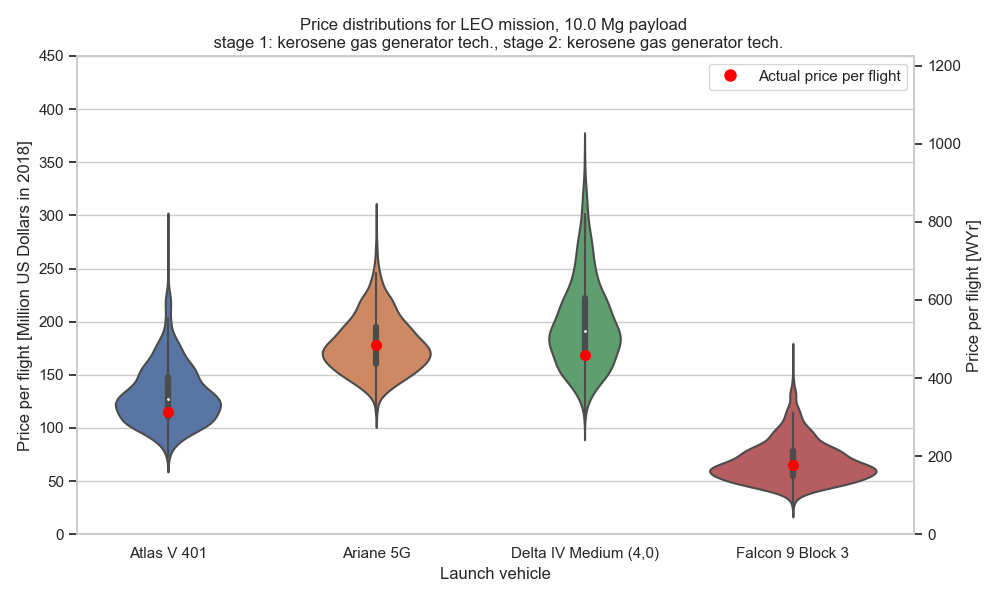
\includegraphics[width=\textwidth]{../../lvreuse/analysis/cost/plots/vehicle_ppf_validation}
    \caption{\label{fig:vehicle_ppf_validation} Distributions of price per flight estimates for several launch vehicles. Available actual price per flight information is included for comparison.}
\end{figure*}

The price estimate distributions for these four vehicles are all reasonable, capturing the actual price per flight near the mode of the distribution. The distribution for Falcon 9 is predictably lower than the others, accounting for its high launch rate and SpaceX's lean manufacturing practices with minimal overhead costs. We see a slightly broader distribution of costs for the Delta IV launch vehicle, likely due to a few reasons. First, its use of the modern RS-68 engine on the first stage -- which has few similar reference projects for fitting of historical data -- requires a relatively broad confidence interval to characterize the CER coefficients. Second, the sensitivity of the launch vehicle costs to its learning factor is larger since the Delta IV is earlier in its program life than the other launch vehicles. These estimates lend credibility to the cost per flight estimates for the various first stage reuse strategies to be shown. 

\section{Discussion}

This section presents estimates of the cost-per-flight of various reuse strategies. Two strategies, (downrange, rocket-propelled, propulsive landing, full recovery) and (downrange, no propulsion, parachute, full recovery), are shown to dominate the other strategies on cost. However, parachute recovery of the full first stage is likely only practical for small launch vehicles\footnote{A small stage on parachutes could be recovered in midair or on a ship, or survive landing on land. A large stage on parachutes may need to land directly in the ocean, which would increase recovery and refurbishment expenses.}, and it will also be shown that first stage reuse is not favorable for small launch vehicles. Thus, downrange propulsive landing appears to be the dominant strategy.

Launch rate is also a critical factor in the economics of reuse. Increasing launch rate further reduces cost-per-flight, and also allows the investment in reuse development to be paid off more quickly. Efficient first stage reuse may allow for an increase in launch rate. A market that can support a high (>20 flights/year) launch rate may be a critical factor for the economic viability of a first stage reuse.

The discussion is organized as follows: the first subsection shows the distribution of cost-per-flight estimates under a generic dispersion of the model input parameters. The subsequent subsections examine the effect of number of reuses, launch rate, and launch vehicle size on cost. Finally, the last section discusses whether the present value of cost savings from reuse is enough to justify the initial investment in its development.

\subsection{Strategy cost-per-flight estimates}

In order to evaluate the cost per flight distributions for various first stage reuse strategies, we again perform a Monte Carlo analysis. This is implemented by evaluating the performance and cost models in sequence, sampling from generic distributions of model input parameters. For a given payload, we first evaluate the required masses of the launch vehicle elements for different reuse strategies using the performance model. Then, those resulting masses are used with the cost model to evaluate the cost per flight of the launch vehicles for each reuse strategy. Some of these cost per flight distributions are shown in Figures \ref{fig:strategy_cost_LEO_kerosene_pld10000}- \ref{fig:strategy_cost_LEO_H2_pld10000}. 

\begin{figure*}
    \centering
    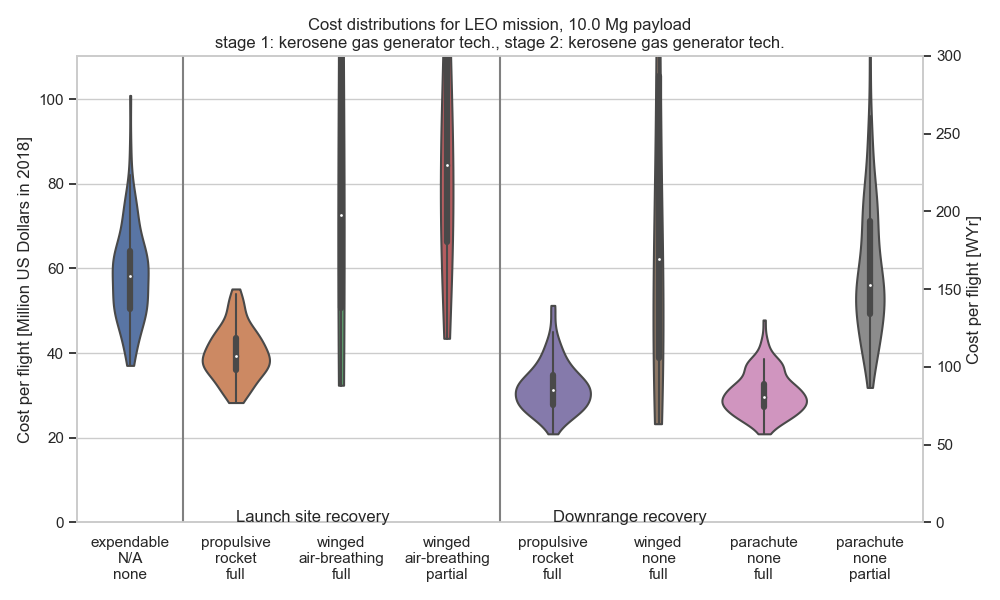
\includegraphics[width=\textwidth]{../../lvreuse/analysis/combined/plots/strategy_cost_LEO_kerosene_pld10000}
    \caption{\label{fig:strategy_cost_LEO_kerosene_pld10000} Cost per flight distributions for various first stage reuse strategies, assuming kerosene technology and carrying a 10 ton payload to LEO. Note that downrange propulsive landing and downrange parachute recovery have the lowest expected costs, and that the cost of winged strategies is highly uncertain.}
\end{figure*}

\begin{figure*}
    \centering
    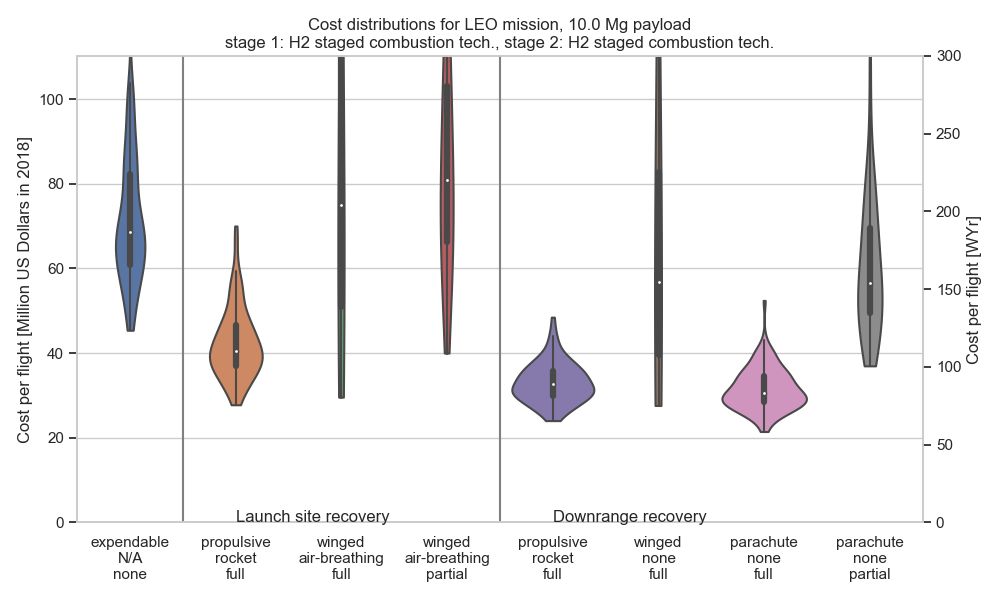
\includegraphics[width=\textwidth]{../../lvreuse/analysis/combined/plots/strategy_cost_LEO_H2_pld10000}
    \caption{\label{fig:strategy_cost_LEO_H2_pld10000} Cost per flight distributions for various first stage reuse strategies, assuming hydrogen technology and carrying a 10 ton payload to LEO. The distributions are similar to those for kerosene, although the expected costs are slightly higher.}
\end{figure*}

The downrange propulsive landing and parachute strategies for full first stage recovery show very similar distributions with the lowest cost per flight distributions among all the strategies. However, as mentioned previously, parachute recovery of the full first stage is not very feasible for large vehicles. Therefore downrange propulsive landing is the most effective strategy for achieving the lowest cost per flight. 

We see broad distributions for winged recovery strategies due to a small number of historical reference projects available for fitting the production CER coefficients. This lack of data leads to large uncertainties in the coefficient values, resulting in large uncertainties in the output cost per flight distributions. 

It is also interesting to compare the cost per flight distributions for the two different technology choices (kerosene with gas generator and H2 with staged combustion). Despite the hydrogen technology choice yielding slightly better payload performance, the cost per flight distributions show slightly lower costs for kerosene. This result likely stems from two reasons:

\begin{itemize}
  \item The cost per kilogram of inert mass for producing a vehicle using hydrogen propellant is greater than that for kerosene. 
  \item The inert mass of a vehicle using hydrogen propellant is generally greater than that of kerosene for a given payload mass.
\end{itemize}

Additionally, partial reuse strategies do not seem to yield substantial cost per flight savings relative to full reuse strategies. For these reuse strategies, the extra mass required to make a first stage vehicle partially recoverable does not make up for any cost savings achieved by reusing the high-value components. 

% Maybe include some GTO stuff here if there is room.

\subsection{Effect of number of reuses and launch rate}
In order to look at the breakdown of costs for a launch vehicle with a reusable first stage, we consider a point cost estimate to demonstrate general trends. The following example evaluates a two stage launch vehicle carrying a 10,000 kg payload to LEO using kerosene and liquid oxygen propellants at a launch rate of 15 launches per year. We consider the case of a propulsive downrange landing to recover and reuse the entire first stage. The cost per flight is determined over a range of number of first stage uses. The results of this analysis are shown in Figure \ref{fig:cpf_stackplot_reuses_sweep}.

\begin{figure}[H]
    \centering
    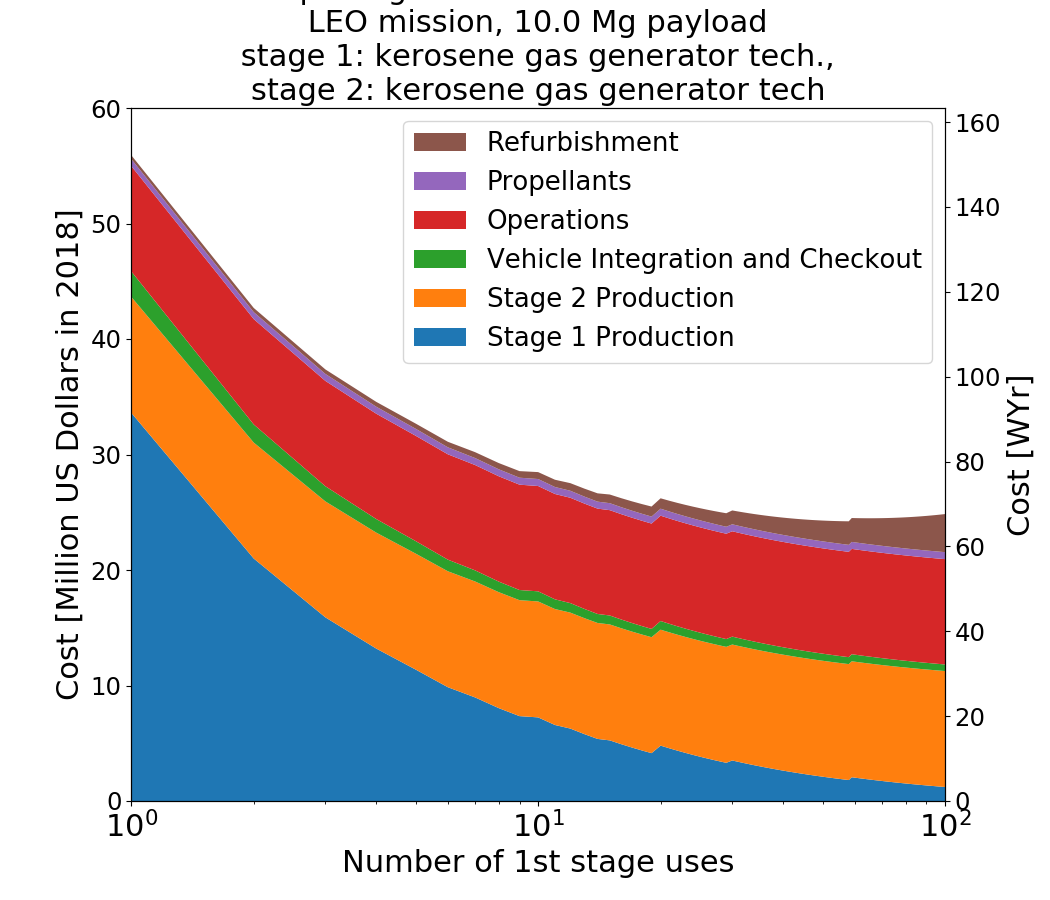
\includegraphics[width=0.5\textwidth]{../../lvreuse/analysis/combined/plots/cpf_stackplot_reuses_sweep}
    \caption{\label{fig:cpf_stackplot_reuses_sweep} A sweep of cost per flight vs number of first stage reuses for an example downrange propulsive landing strategy. Stage 1 production cost per flight declines as the first stage is reused more times. Refurbishment costs make up a small fraction of the cost per flight, but increase with increasing number of reuses.}
\end{figure}

Several things should be noticed from the results in Figure \ref{fig:cpf_stackplot_reuses_sweep}. First, the stage one productions costs per flight decrease dramatically as we increase the number of first stage reuses. This result is very intuitive -- as the cost of first stage production is spread over a larger number of flights, the per flight amortization share of the first stage production cost decreases. This leads to a reduction in the cost per flight. However, this trend of decreasing amortization share of first stage production costs is opposed by the refurbishment cost trends. As the number of first stage uses increases, the refurbishment cost per flight also increases. This is due to the fact that more components on the first stage will need inspected or replaced  as the number of reuses increases. 

These opposing trends lead to an interesting result: the total cost per flight trend achieves a minimum value. Under the assumptions used in Figure \ref{fig:cpf_stackplot_reuses_sweep}, the minimum cost per flight occurs near 60 reuses, but the exact location is highly dependent the model parameters, especially refurbishment costs. Generally though, there will be some number of reuses beyond which further reuse is not cost effective.

The cost per flight is also affected by the annual launch rate. Although most components of the cost per flight do not vary with launch rate, operations costs are very sensitive to it. Launch operations require a dedicated workforce and facilities, which are underutilized at low launch rates. Therefore we see a higher operations cost per flight at low launch rates. The cost per flight trends with varied launch rates are given in Figure \ref{fig:cpf_reuses_sweep_vary_launch_rate}. 

\begin{figure}[H]
    \centering
    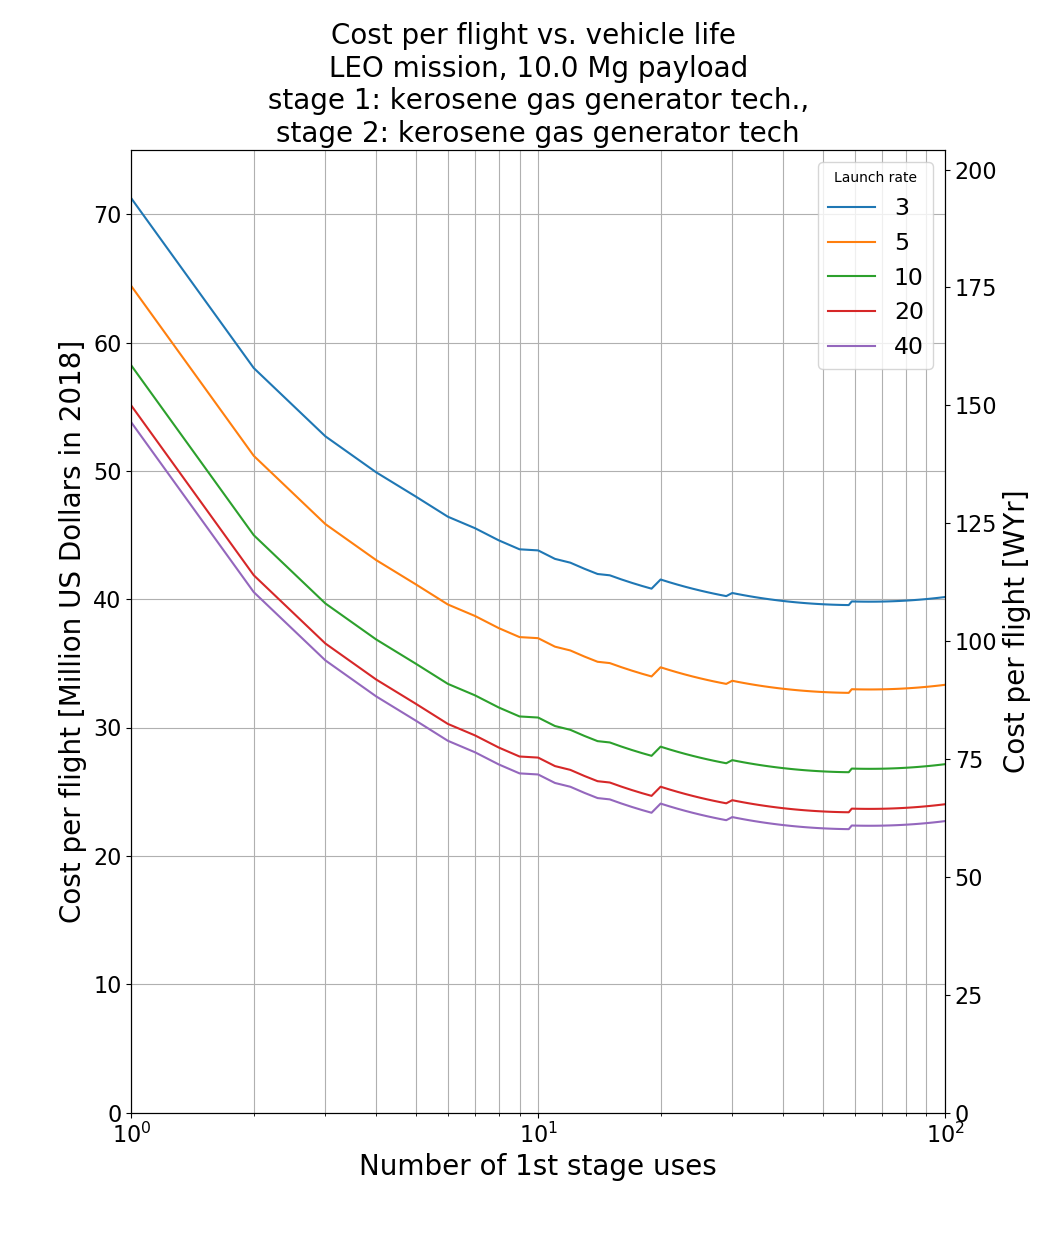
\includegraphics[width=0.5\textwidth]{../../lvreuse/analysis/combined/plots/cpf_reuses_sweep_vary_launch_rate}
    \caption{\label{fig:cpf_reuses_sweep_vary_launch_rate} The cost per flight vs. number of reuses sweep repeated at several launch rates. Increasing launch rate decreases cost per flight (primarily through lower operational costs) but the benefits diminish past about 20 launches/year.}
\end{figure}

As expected, Figure \ref{fig:cpf_reuses_sweep_vary_launch_rate} shows that the cost per flight is higher at lower launch rates, regardless of the number of first stage reuses. For low launch rates, we see a substantial decrease in the cost per flight for only a modest increase in launch rate. However, for high launch rates, further increases in launch rate do not have a large effect on the cost per flight. For instance, we see a large difference in cost per flight by increasing the launch rate from 3 to 5 launches per year. However, increasing the launch rate from 20 to 40 launches per year yields only minimal cost per flight reductions. 

We next consider some of these cost per flight trends for various first stage reuse strategies. Figure \ref{fig:num_reuse_sweep_LEO_kerosene} shows the costs per flight for selected strategies over a range of number of first stage uses. We consider two cases in this analysis: 

\begin{itemize}
  \item First stage reuse has no effect on the vehicle launch rate. The first stage production rate is not a rate-limiting step of the launch rate. In this case, a production and launch rate of 15 vehicles per year. 
  \item First stage reuse allows the launch rate to increase beyond the first stage production rate. For illustration, we assume that the first stage production rate is 15 stages per year, and that in this case the launch rate is $min(15 * n_{reuse}, 50)$
\end{itemize}

For all strategies, we see a decrease in the cost per flight as the number of first stage uses increases. This result is not surprising -- increasing the launch rate decreases the operations cost per flight. It is interesting though to compare the strategy cost per flight trends with the cost of an expendable vehicle. For the strategies considered in Figure \ref{fig:num_reuse_sweep_LEO_kerosene}, all but the partial parachute recovery strategy show costs per flight below the 10th percentile of expendable cost per flight estimates above a certain number of reuses. With partial parachute recovery, the high-value hardware reuse savings do not compensate for the additional costs of producing and operating a reusable vehicle. However, the other strategies show potential for significant cost per flight savings with a high enough number of first stage reuses. 

\begin{figure*}
    \centering
    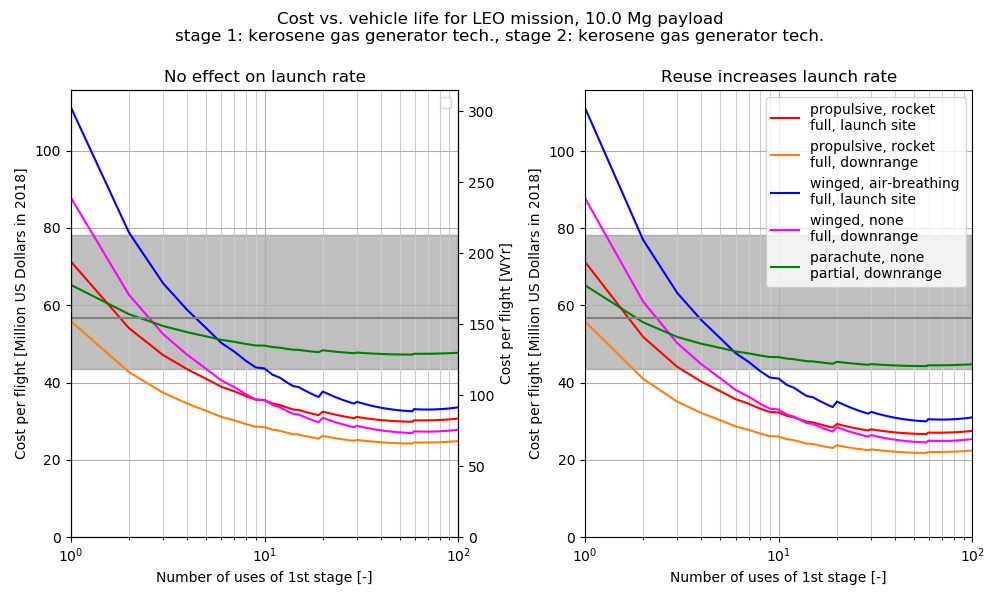
\includegraphics[width=\textwidth]{../../lvreuse/analysis/combined/plots/num_reuse_sweep_LEO_kerosene}
    \caption{\label{fig:num_reuse_sweep_LEO_kerosene} The cost per flight vs. number of reuses sweep, repeated for various reuse strategies. For comparison, the grey bar shows the expendable cost distribution's \nth{10} to \nth{90} percentiles.}
\end{figure*}

\subsection{Effect of launch vehicle size}

The potential for cost per flight savings of first stage reusability is highly dependent on the payload or vehicle size. In the previous discussion, we considered the case of a 10 Mg payload to LEO. The cost per flight breakdown for this case shown in Figure \ref{fig:cpf_stackplot_reuses_sweep} shows that first stage production costs make up the majority of costs in the expendable case, and that first stage reuse can lead to significant cost per flight savings. However, the cost per flight breakdown looks very different for a smaller payload. 

Let's consider the case of a small 100 kg payload to LEO. As can be seen in Figure \ref{fig:cpf_stackplot_reuses_sweep_small_sat}, first stage production costs no longer make up the majority of the cost per flight since costs for small launch vehicles are not dominated by hardware costs. Instead, the operations costs make up the majority of the cost per flight. The operations costs per flight are largely independent of vehicle and payload mass, and therefore do not decrease substantially as the payload and vehicle mass decrease. For these reasons, first stage reusability for small launch vehicles is impractical. Amortizing the first stage production costs for a small launch vehicle over a number of flights does not lead to large cost per flight savings since the production costs were already a small fraction of the cost per flight.

\begin{figure}[H]
    \centering
    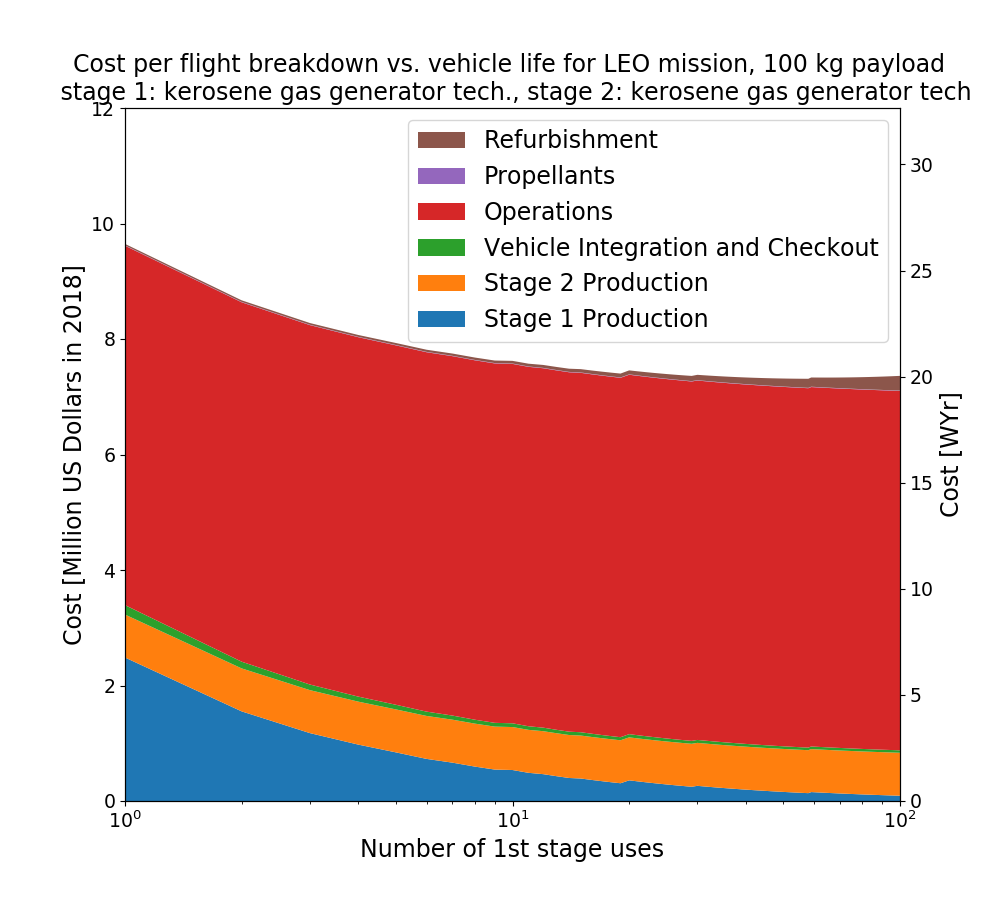
\includegraphics[width=0.5\textwidth]{../../lvreuse/analysis/combined/plots/cpf_stackplot_reuses_sweep_small_sat}
    \caption{\label{fig:cpf_stackplot_reuses_sweep_small_sat} The cost per flight of a small launcher (100 kg payload) is expected to be dominated by operations costs, and does not decline meaningfully with first stage reuse.}
\end{figure}

We next consider the cost per kilogram payload per flight over a range of payload masses, as given in Figure \ref{fig:m_payload_sweep_LEO_kerosene}. This plot reveals a trend of decreasing cost per kilogram payload per flight as payload mass -- and therefore vehicle size -- increases. More interesting though is that the spread between the estimates of cost per kilogram payload per flight increases with increasing payload mass and launch vehicle size. 

As previously discussed, the cost per flight for small vehicles is not dominated by vehicle hardware costs. Even though there are differences in payload mass fractions (TODO ref performance section/violin plots) between strategies, these differences are relatively inconsequential in estimating cost per flight for small vehicles since hardware mass was not a strong cost driver anyway. However, for increasing payload vehicle size, hardware costs make up a larger fraction of the cost per flight. Therefore, as the vehicle size increases, we see the cost per flight per mass payload estimates for the different reuse strategies diverge as differences in payload performance become more important in determining costs. 

\begin{figure}[H]
    \centering
    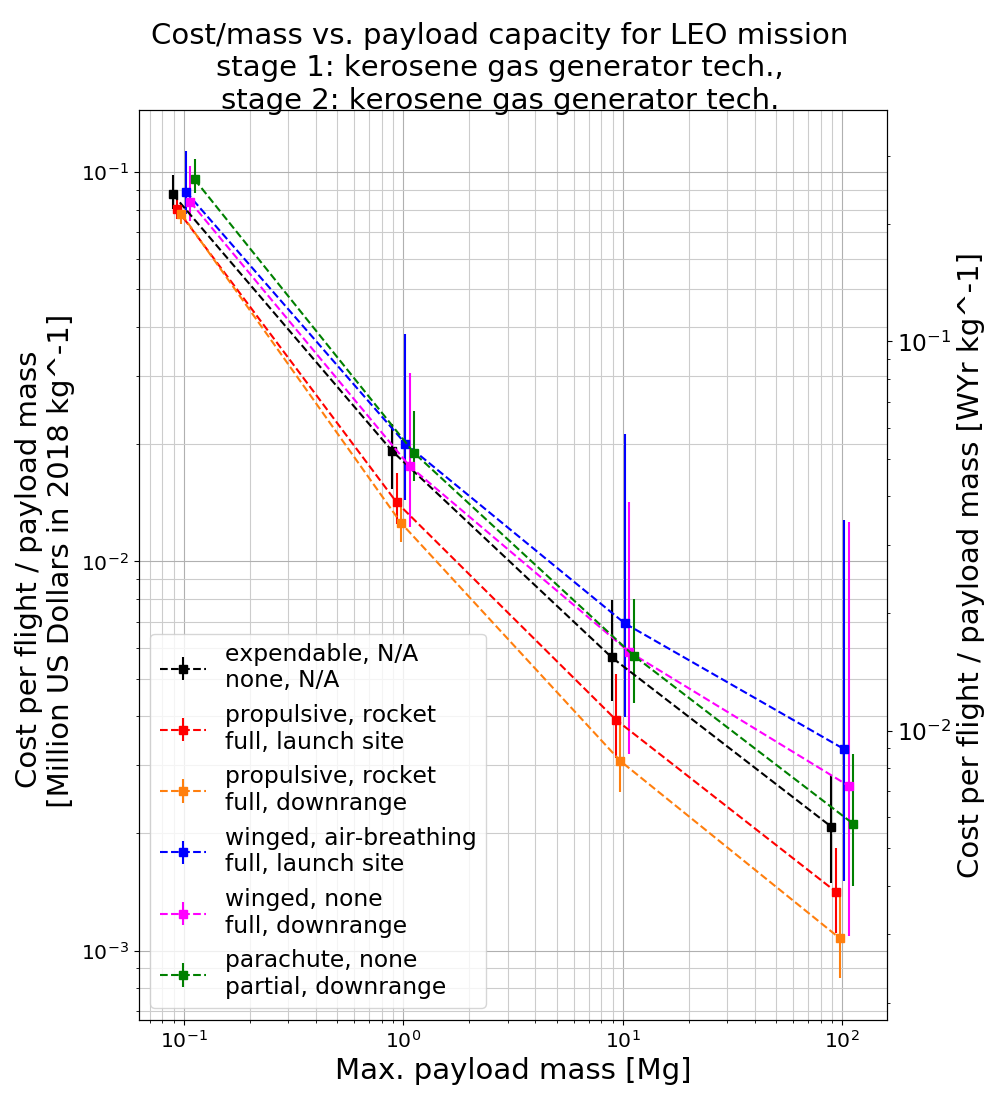
\includegraphics[width=0.5\textwidth]{../../lvreuse/analysis/combined/plots/m_payload_sweep_LEO_kerosene}
    \caption{\label{fig:m_payload_sweep_LEO_kerosene} As payload mass increases, the cost/mass spread between reuse strategies widens. The error bars on each point show the \nth{10} to \nth{90} percentiles of the cost/mass estimate. The points are "jittered" on the x-axis for visual clarity.}
\end{figure}

\subsection{Paying off development costs}

In our models and discussion so far, we have yet to consider the development costs of the reuse strategies. The development costs of reusable launch vehicles can generally be expected to be greater than a similar expendable vehicle. However, the cost per flight savings for reusable vehicles can also be substantial, as shown in Figure \ref{fig:num_reuse_sweep_LEO_kerosene}. These opposing trends lead to an important question: do the cost per flight savings of reusable launch vehicles pay off their increased development costs? 

We address this question by comparing the present value of the savings brought by reusability to the reusable vehicle development costs. In Figure \ref{fig:reuse_npv}, we evaluate the present value of the savings for different launch rates over a range of cost per flight ratios, or the ratio between the cost per flight of a vehicle with first stage reuse and the cost per flight of an expendable vehicle. Credible ranges of development costs and cost per flight ratios are highlighted.

The vehicle launch rate determines how quickly the cost per flight savings for reusability are accrued. With higher launch rates, savings are realized sooner, the present value of the savings is larger, and the investment in reuse development can be paid off faster. This is why we see steeper trends for the present value of savings with higher launch rates. 

In order for a strategy to be economically viable, the present value of the savings must exceed the vehicle's development costs. This seems unlikely for low launch rates -- savings will be realized slowly such that development costs will be greater than the present value of the savings. However, for high launch rates greater than 20 launches per year, first stage reusability appears economically viable. Increased launch rates both reduce the cost per flight and enable the development investment to be paid off sooner. This leads to a higher present value of reuse cost per flight savings, such that the development costs could feasibly be paid off.

\begin{figure}[H]
    \centering
    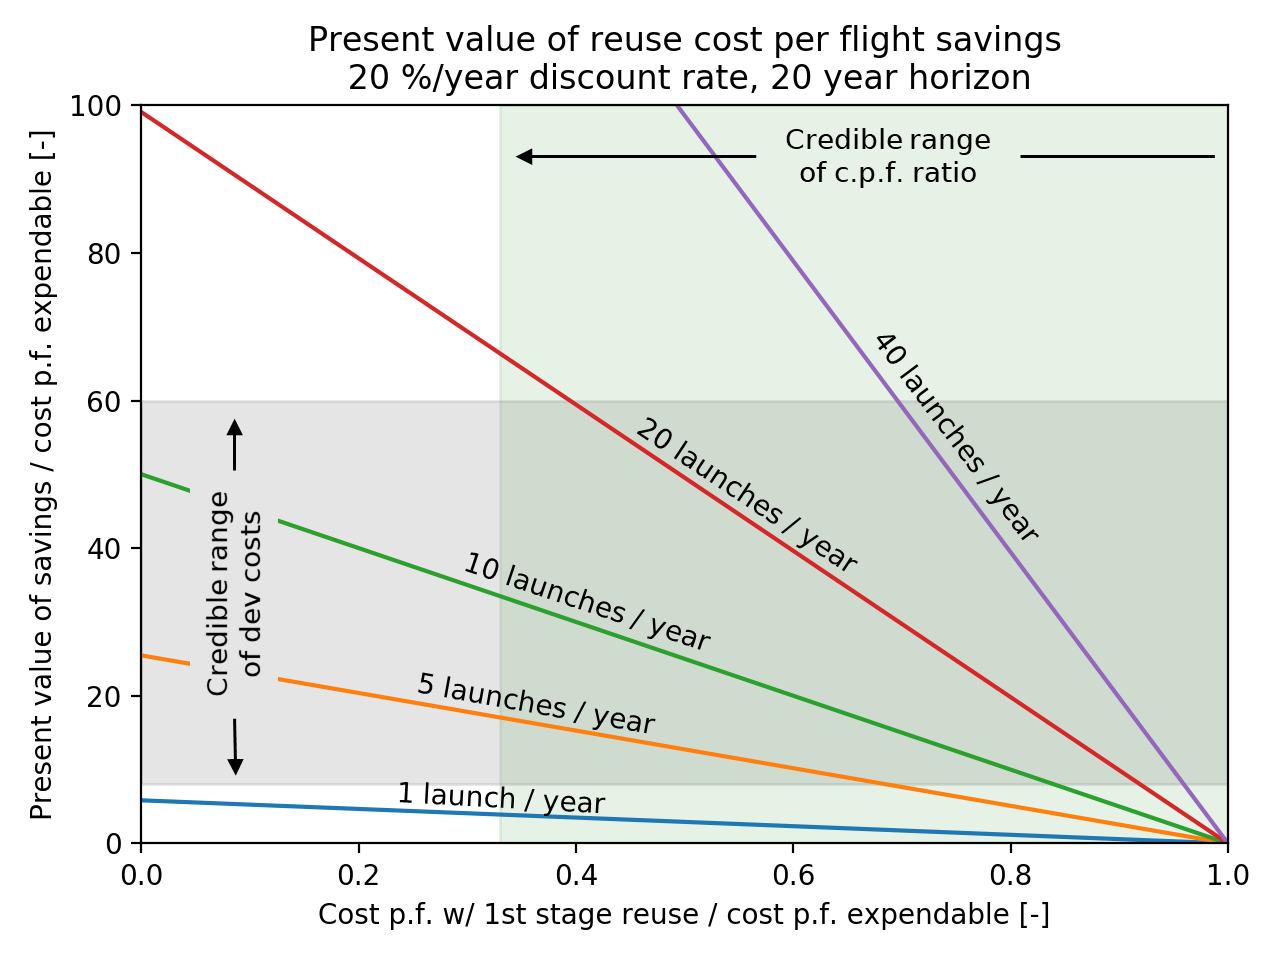
\includegraphics[width=0.5\textwidth]{reuse_npv}
    \caption{\label{fig:reuse_npv} The present value of the cost savings from reuse is higher at higher launch rates.}
\end{figure}

\section{Conclusion}

This paper has introduced preliminary models for the performance and cost of launch vehicles employing various strategies for first stage reuse. We used Monte Carlo techniques to evaluate these models while taking into account uncertainty in the model input parameters.

Winged reuse strategies were found to have very uncertain and likely high costs, and partial reuse strategies did not offer meaningful cost savings. In contrast, downrange propulsive landing offers significant cost savings and is probably the dominant strategy from a cost per flight standpoint. It could plausibly reduce launch costs to $\frac{1}{2}$ to $\frac{1}{3}$ the cost of an expendable vehicle.

Reuse makes most sense for large launch vehicles with high launch rates. A small sizes, the first stage hardware costs are only a small fraction of the cost per flight, so reuse is not particularly helpful. High launch rates (>20/year) are likely required to pay off the development costs of reuse. However, first stage reuse may facilitate higher launch rates if first stage production is the rate limiting step. Further, interest in high-count LEO constellations indicates that the market demand may be sufficient to sustain these high launch rates. Thus, the present analysis indicates that first stage reuse is a viable route to reducing launch costs for medium to heavy lift launch vehicles.

\bibliography{first_stage_recovery}
\end{multicols}
\end{document}
